\documentclass[10pt]{article}
\usepackage{puconf}

\begin{document}
\twocolumn[{
\begin{@twocolumnfalse}
\begin{center}
\begin{minipage}{0.86\textwidth}
\centering
\rule{\linewidth}{2.4pt}
\vspace{9pt}

{\fontsize{19.5}{22.0}\selectfont\bfseries
PU-Boost: A Two-Stage Reliable-Sample Reconstruction Positive-Unlabeled Learning Framework for Screening Undiagnosed Hypertension\par}

\vspace{8pt}
\rule{\linewidth}{1.25pt}
\end{minipage}
\end{center}
\vspace{10pt}

\begin{center}
\begin{minipage}[t]{0.235\textwidth}\centering
{\normalsize\bfseries Huanqi Wu\textsuperscript{1,*}}\\[-1pt]
{\footnotesize\texttt{huanqiwu@arizona.edu}}
\end{minipage}\hfill
\begin{minipage}[t]{0.235\textwidth}\centering
{\normalsize\bfseries Liangkun Shi\textsuperscript{1}}\\[-1pt]
{\footnotesize\texttt{liangkuns@arizona.edu}}
\end{minipage}\hfill
\begin{minipage}[t]{0.235\textwidth}\centering
{\normalsize\bfseries Hanfei Yang\textsuperscript{1}}\\[-1pt]
{\footnotesize\texttt{yanghanfei@arizona.edu}}
\end{minipage}\hfill
\begin{minipage}[t]{0.235\textwidth}\centering
{\normalsize\bfseries Lizhu Guo\textsuperscript{2}}\\[-1pt]
{\footnotesize\texttt{azguolizhu@gmail.com}}
\end{minipage}

\vspace{7pt}
{\footnotesize
\textsuperscript{1}Department of Mathematics, University of Arizona, Tucson, AZ 85721, USA\\
\textsuperscript{2}Department of Cardiology, Beijing Anzhen Hospital, Capital Medical University, Beijing, China}

\end{center}

\vspace{7pt}
\begin{center}
\begin{minipage}{0.90\textwidth}
\noindent\textbf{Abstract.} In hypertension screening, previously diagnosed cases provide reliable
positive labels, whereas individuals without a prior diagnosis comprise
both undiagnosed hypertensive and non-hypertensive individuals, creating
a canonical positive-unlabeled (PU) learning setting. We propose
PU-Boost, a two-stage reliable-sample reconstruction framework that uses
only readily obtainable demographic, behavioral, medical-history, and
anthropometric variables. During training, only previously diagnosed
hypertension cases are treated as labeled positives (P), while all
remaining individuals are treated as unlabeled (U); no additional
reference labels are supplied to the two-stage reconstruction procedure.
Elastic Net first provides a global ranking of P versus U, after which a
random forest refines the uncertain region and highly ambiguous
observations are rejected. XGBoost is then trained on the reconstructed
class-balanced pseudo-labeled sample. In the independent test set,
PU-Boost achieved a sensitivity of 0.817 and a balanced accuracy of
0.682, the highest observed values among the compared models. It
produced 729 false negatives, 41.1\% fewer than standard XGBoost,
although specificity decreased to 0.547. SHAP analysis indicated that
established hypertension-related features, including age, body mass
index, waist circumference, and family history, contributed strongly to
model output. PU-Boost therefore provides a statistically motivated
framework for reducing missed cases when screening for undiagnosed
hypertension under incomplete diagnostic labeling.

\vspace{3pt}
\noindent\textbf{Keywords:} Positive-unlabeled learning; Hypertension screening; Reliable sample reconstruction; Weak supervision; Machine learning; Risk stratification
\end{minipage}
\end{center}
\vspace{7pt}
\end{@twocolumnfalse}
}]

\section{Introduction}

Hypertension is a major global public-health challenge and an important
risk factor for cardiovascular disease, stroke, chronic kidney disease,
and premature mortality(Collaboration, 2021; Oparil et al., 2018; World
Health Organization, 2025). Although hypertension can be identified
directly through blood-pressure measurement, a substantial proportion of
affected individuals remain undiagnosed in real-world settings,
particularly during earlier stages when symptoms are often absent(World
Health Organization, 2025). National hypertension surveys in China
indicate that prevalence remains high while awareness, treatment, and
control remain suboptimal(Cao et al., 2025; Wang et al., 2018).
Undiagnosed hypertension may delay timely intervention and increase the
long-term burden on health-care systems. Accordingly, identifying
high-risk individuals using simple and readily available information is
an important objective in hypertension prevention and management.

Machine-learning methods have increasingly been used for hypertension
risk prediction and disease screening. Previous studies have developed
predictive models from demographic characteristics, lifestyle factors,
anthropometric measures, and electronic health records using logistic
regression, random forests, gradient boosting, and neural
networks(Chowdhury et al., 2022; Silva et al., 2022). However, when
training labels are constructed solely from prior diagnosis,
conventional supervised classifiers typically treat previously diagnosed
individuals as positives and everyone else as non-positive(Chang et al.,
2022). If hidden positives are present among those without a prior
diagnosis, the observable label S differs from the reference disease
status Y(Chang et al., 2022; Elkan \& Noto, 2008). Consequently,
minimizing empirical loss with respect to S targets a quantity closer to
Pr(S=1\textbar X) than to the screening target Pr(Y=1\textbar X). This
target mismatch causes undiagnosed reference-positive individuals to
contribute negative supervision and can distort the learned decision
boundary. Based on prior diagnosis and reference disease status,
participants can be classified retrospectively into three groups: group
A, diagnosed hypertension; group B, undiagnosed hypertension; and group
C, non-hypertensive individuals. The A/B/C grouping is used to describe
the reference label structure, to support model selection in the
validation set, and to evaluate final performance. During the two-stage
PU reconstruction itself, only group A is observed as a reliable
positive class, whereas the reference identities of groups B and C are
hidden and jointly form the unlabeled population. Direct blood-pressure
measurements are used only to construct Y and for downstream validation
and evaluation, and are not included among the predictors. Thus, hidden
reference-positive and reference-negative individuals may overlap
extensively in the available feature space. The central modeling problem
is therefore not simply to increase classifier complexity, but to
identify high-confidence observations within the unlabeled population
while progressively restricting the region of label uncertainty without
accessing B/C reference identities.

\begin{figure*}[!t]
\centering
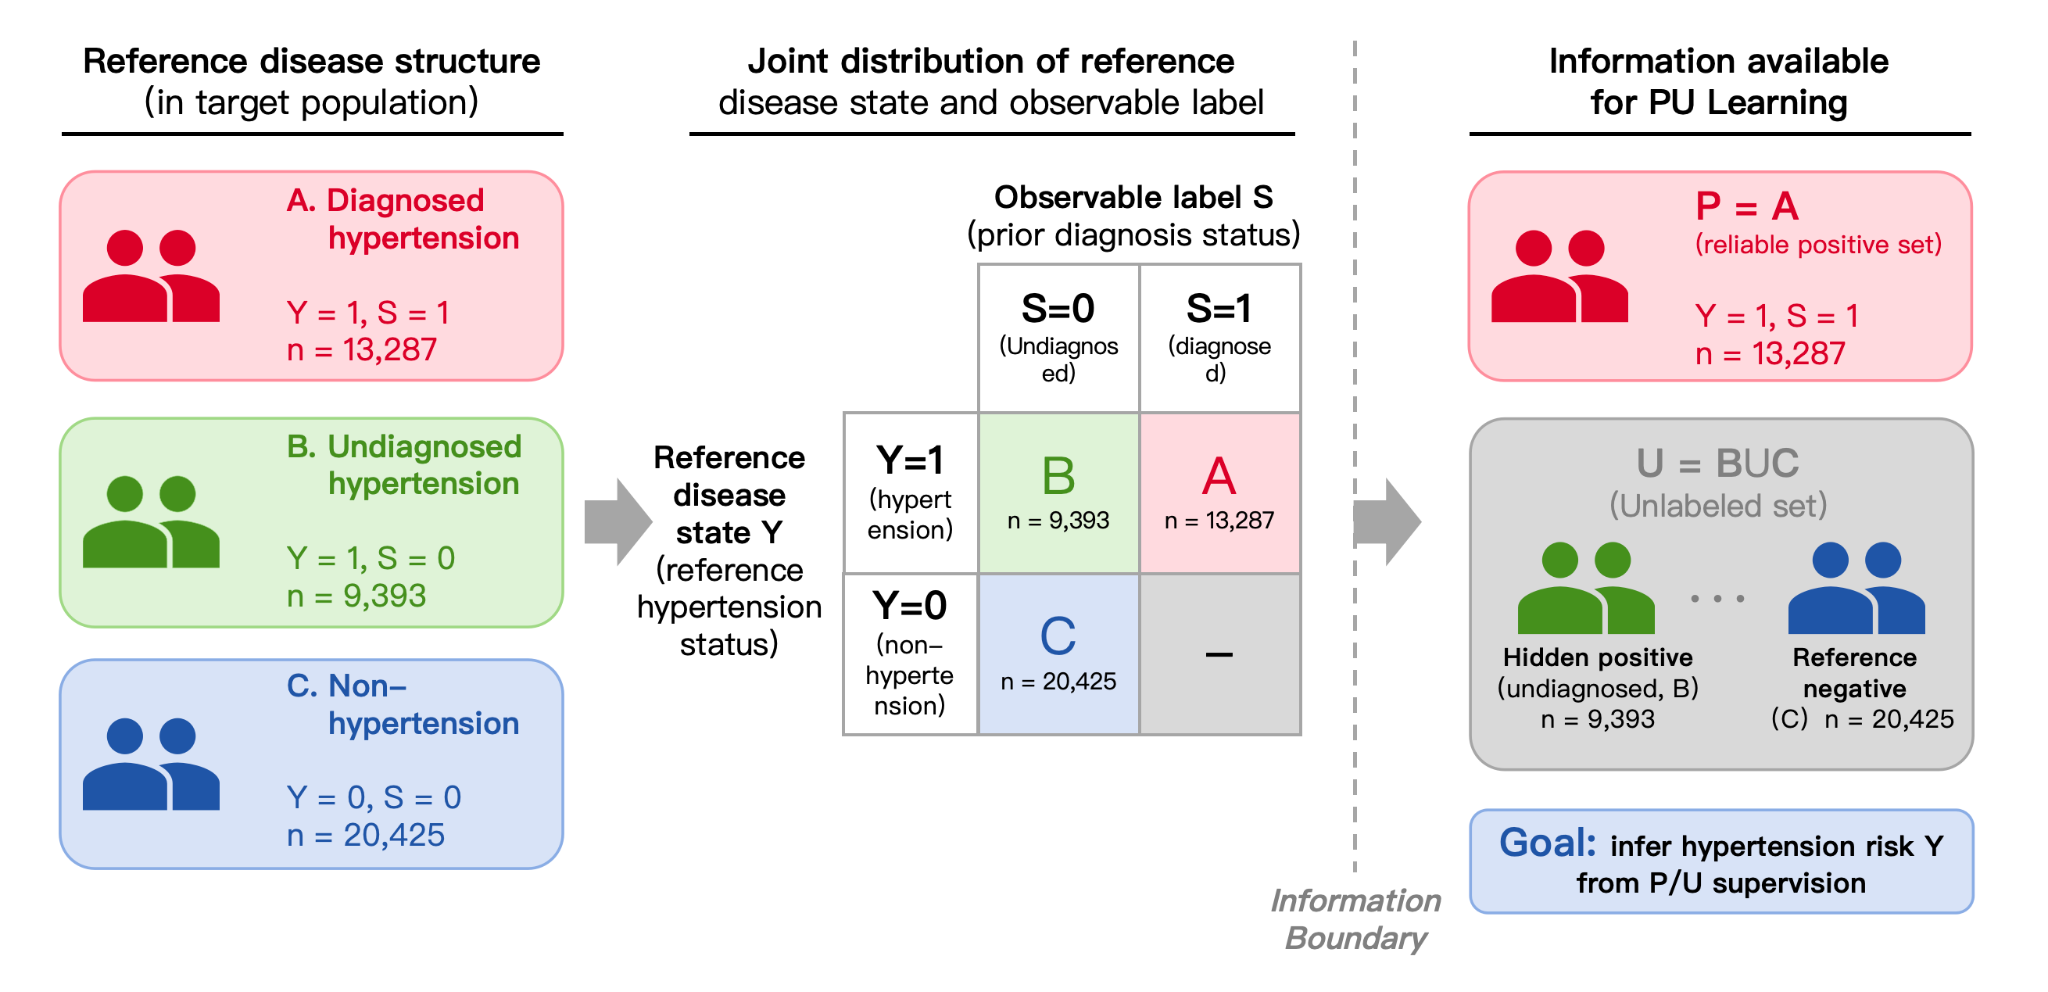
\includegraphics[width=0.97\textwidth]{figures/figure1_reference_structure.png}
\caption{\textbf{Reference disease structure and information available during positive-unlabeled learning.} Participants were retrospectively classified as diagnosed hypertension (group A; Y=1, S=1), undiagnosed hypertension (group B; Y=1, S=0), and non-hypertensive (group C; Y=0, S=0). During two-stage PU reconstruction, only group A was observed as the labeled-positive set P, whereas groups B and C were indistinguishable to the training algorithm and jointly formed the unlabeled set U. Reference B/C identities were used only outside the reconstruction procedure for model selection and performance evaluation.}
\label{fig:reference-structure}
\end{figure*}

Positive-unlabeled (PU) learning addresses classification problems in
which reliable positive examples are available but the remaining
observations are unlabeled(Bekker \& Davis, 2020; du Plessis et al.,
2014; Elkan \& Noto, 2008). Let P denote the labeled-positive set and U
the unlabeled set. Samples in P carry an observed positive label,
whereas the latent class membership of U is unknown and U contains both
hidden positives and negatives. The training-information structure in
this study follows this setting: $P=A$ and $U=B\cup C$, with B/C reference
identities unavailable to the training algorithm. Screening for
undiagnosed hypertension can therefore be naturally formulated as a
PU-learning problem. Unlike conventional supervised learning that treats
U as a negative class, PU learning seeks to exploit information in P and
the mixed unlabeled set U to construct a decision rule informative about
the reference disease state(Bekker \& Davis, 2020; du Plessis et al.,
2015; Kiryo et al., 2017).

PU learning has been applied to cancer prediction,
Alzheimer\textquotesingle s disease identification, and other
disease-screening tasks, but its use for screening undiagnosed
hypertension using only readily available demographic, lifestyle,
medical-history, and anthropometric variables remains limited(Li et al.,
2022; Tran et al., 2025; Wu et al., 2023; Zhou et al., 2022). In the
present setting, the challenge arises not only from the absence of
explicit negative labels but also from substantial overlap within U. A
single-stage procedure that assigns pseudo-labels to all unlabeled
observations may force highly uncertain samples near the decision
boundary into either class and propagate pseudo-label error to the
downstream classifier(Bekker \& Davis, 2020; Hendrickx et al., 2024; Liu
et al., 2002). We therefore focus on progressively identifying
high-confidence candidate samples from U while allowing persistently
ambiguous observations to remain unassigned and limiting their
contribution to the final supervised loss.

Using data from 43,105 community-dwelling adults aged $\geq$45 years across
eight study areas in China, we develop PU-Boost, a two-stage PU-learning
framework. In stage 1, Elastic Net logistic regression produces a
regularized P-versus-U discrimination score for global stratification
into high-confidence candidate positives, candidate negatives, and an
uncertain region. In stage 2, a random forest is applied only to the
stage-1 uncertain region to exploit nonlinear structure and
interactions, yielding additional candidate positives, candidate
negatives, and a highly ambiguous subset that is excluded from final
classifier training. The retained high-confidence candidates are then
assembled into a balanced pseudo-labeled training set and used to train
XGBoost as the final classifier. The architecture progressively
restricts uncertain supervision through global stratification, local
nonlinear refinement, and uncertainty rejection.

This study makes three main contributions. First, it formalizes
screening for undiagnosed hypertension as a PU-learning problem and
explicitly distinguishes the observable diagnosis label from the
reference disease status. Second, it introduces a two-stage
reliable-sample reconstruction strategy combining global stratification,
local nonlinear refinement, and rejection of persistently uncertain
observations, thereby avoiding forced pseudo-label assignment for the
entire unlabeled set. Third, it evaluates the screening operating
characteristics of the resulting model in an independent test set, with
particular emphasis on sensitivity, false negatives, specificity,
balanced accuracy, and model interpretability, and compares these
characteristics with conventional supervised-learning baselines.

\section{Methods}

\subsection{Study population and data
source}\label{study-population-and-data-source}

This study used data from a nationally representative, cross-sectional,
community-based survey conducted in China between 2014 and 2016(Du et
al., 2021). The original survey used a two-stage stratified
cluster-sampling design, with sampling sites in Jilin, Xinjiang,
Beijing, Henan, Jiangxi, Zhejiang, Guangdong, and Yunnan, covering seven
major geographic regions of China: Northeast, Northwest, North, Central,
East, South, and Southwest. Data collection was completed for 47,841
adults aged $\geq$45 years, of whom 43,105 met the analytic inclusion
criteria for the present study. The survey collected demographic
characteristics, lifestyle and behavioral factors, medical history,
medication information, blood-pressure measurements, laboratory
measures, and anthropometric indices. The sampling design, measurement
procedures, and data-collection protocol of the original survey have
been described previously(Du et al., 2021). The study protocol was
approved by the Ethics Committee of Beijing Anzhen Hospital, and all
participants provided written informed consent.

\subsection{Predictors and data
preprocessing}\label{predictors-and-data-preprocessing}

The study was designed to develop a screening model for risk
stratification before confirmatory blood-pressure measurement.
Predictors were therefore restricted to demographic characteristics,
lifestyle factors, general medical history, and anthropometric measures
that are relatively easy to obtain at the population level. Medication
information, laboratory measurements, and blood-pressure measurements
used to define the reference hypertension status were excluded from
model inputs. Following problem-oriented variable screening, 60
predictors were retained from approximately 320 original candidate
variables for model development.

To prevent information leakage, all preprocessing steps requiring
estimation from the data distribution were performed within the training
set and then applied unchanged to the validation and test sets.
Observations with missing values in variables required for model
development were excluded using complete-case analysis. Continuous
variables were standardized using parameters estimated from the training
set. Categorical variables were represented by dummy (indicator)
variables with one level designated as the reference category; category
levels and encoding rules were defined from the training data and
applied consistently to the validation and test sets.

\subsection{Definition of hypertension status and label
groups}\label{definition-of-hypertension-status-and-label-groups}

The reference hypertension status was defined jointly from prior
diagnosis of hypertension and standardized blood-pressure measurements
obtained during the survey. Under the original survey protocol, each
participant underwent three blood-pressure measurements. Let
\(SBP_{im}\) and \(DBP_{im}\) denote the systolic and diastolic blood
pressure, respectively, for participant \(i\) at measurement \(m\),
where \(m = 1,2,3\). The participant-level representative blood
pressures were defined as the means of the three measurements:

\[{\overline{SBP}}_{i} = \frac{1}{3}\sum_{m = 1}^{3}SBP_{im},\quad\quad{\overline{DBP}}_{i} = \frac{1}{3}\sum_{m = 1}^{3}DBP_{im}.\]

Following the hypertension criterion used in the original survey (Du et
al., 2021; Revision., 2019)(systolic blood pressure 140 mmHg; diastolic
blood pressure 90 mmHg), define the measured elevated-blood-pressure
indicator \(H_{i}\):

\[H_{i}= \mathbb{I}\left( {\overline{SBP}}_{i} \geq 140\ \text{or}\ {\overline{DBP}}_{i} \geq 90 \right).\]

Define the prior-diagnosis indicator \(D_{i} \in \{ 0,1\}\): if
participant i had previously received a diagnosis of hypertension, then
\(D_{i} = 1\); otherwise \(D_{i} = 0\). Antihypertensive medication use
was not treated as an independent criterion for the reference label.
Direct blood-pressure measurements were used only to construct the
reference disease status and for subsequent performance evaluation and
were not included as model predictors.

Based on the combination of \(D_{i}\) and \(H_{i}\), participants were
retrospectively divided into three reference groups:

\[
\begin{aligned}
A &= \{i:D_i=1\},\\
B &= \{i:D_i=0,\ H_i=1\},\\
C &= \{i:D_i=0,\ H_i=0\}.
\end{aligned}
\]

Group A comprised participants with previously diagnosed hypertension;
group B comprised participants without a prior diagnosis whose measured
blood pressure met the hypertension criterion; and group C comprised
participants without a prior diagnosis whose measured blood pressure did
not meet the hypertension criterion. In the complete analytic cohort,
groups A, B, and C contained 13,287, 9,393, and 20,425 participants,
respectively.

Define the reference disease status \(Y_{i} \in \{ 0,1\}\):

\[Y_{i}= \mathbb{I}\left( D_{i} = 1\ \text{or}\ H_{i} = 1 \right) = \left\{ \begin{matrix}
1, & i \in A \cup B, \\
0, & i \in C.
\end{matrix} \right.\ \]

Unlike \(Y_{i}\), the observable training label \(S_{i}\) records only
prior diagnosis status:

\[S_{i} = D_{i} = \left\{ \begin{matrix}
1, & i \in A, \\
0, & i \in B \cup C.
\end{matrix} \right.\ \]

Thus, the three reference groups correspond to label structures
\(A:(Y = 1,S = 1)\), \(B:(Y = 1,S = 0)\), and \(C:(Y = 0,S = 0)\). The
reference identities of groups B and C are used only outside the
two-stage reconstruction procedure, including model selection,
verification, and performance evaluation, and are not provided as inputs
to PU-Boost during the two-stage training process. The labeled-positive
set \(P\) and unlabeled set \(U\) used for training are defined as

\[P = \{ i:S_{i} = 1\} = A,\quad\quad U = \{ i:S_{i} = 0\} = B \cup C.\]

Therefore, \(S_{i} = 1 \Rightarrow Y_{i} = 1\), whereas \(S_{i} = 0\)
contains both reference-positive and reference-negative individuals.

\subsection{Dataset partitioning and information
isolation}\label{dataset-partitioning-and-information-isolation}

The 43,105 participants were randomly divided in a 6:2:2 ratio into
training, validation, and test sets containing 25,883, 8,611, and 8,611
participants, respectively. Two-stage PU reconstruction was performed
only in the training set, and the training algorithm accessed only the
\(S\)-defined \(P/U\) information. The reference disease status \(Y\) in
the validation set was used only for model selection and hyperparameter
comparison and did not contribute to training-sample reconstruction; the
test set was used only for final performance evaluation after model
specification was fixed. This information separation prevented B/C
reference identities from entering the two-stage PU-Boost fitting
procedure.

\begin{figure*}[!t]
\centering
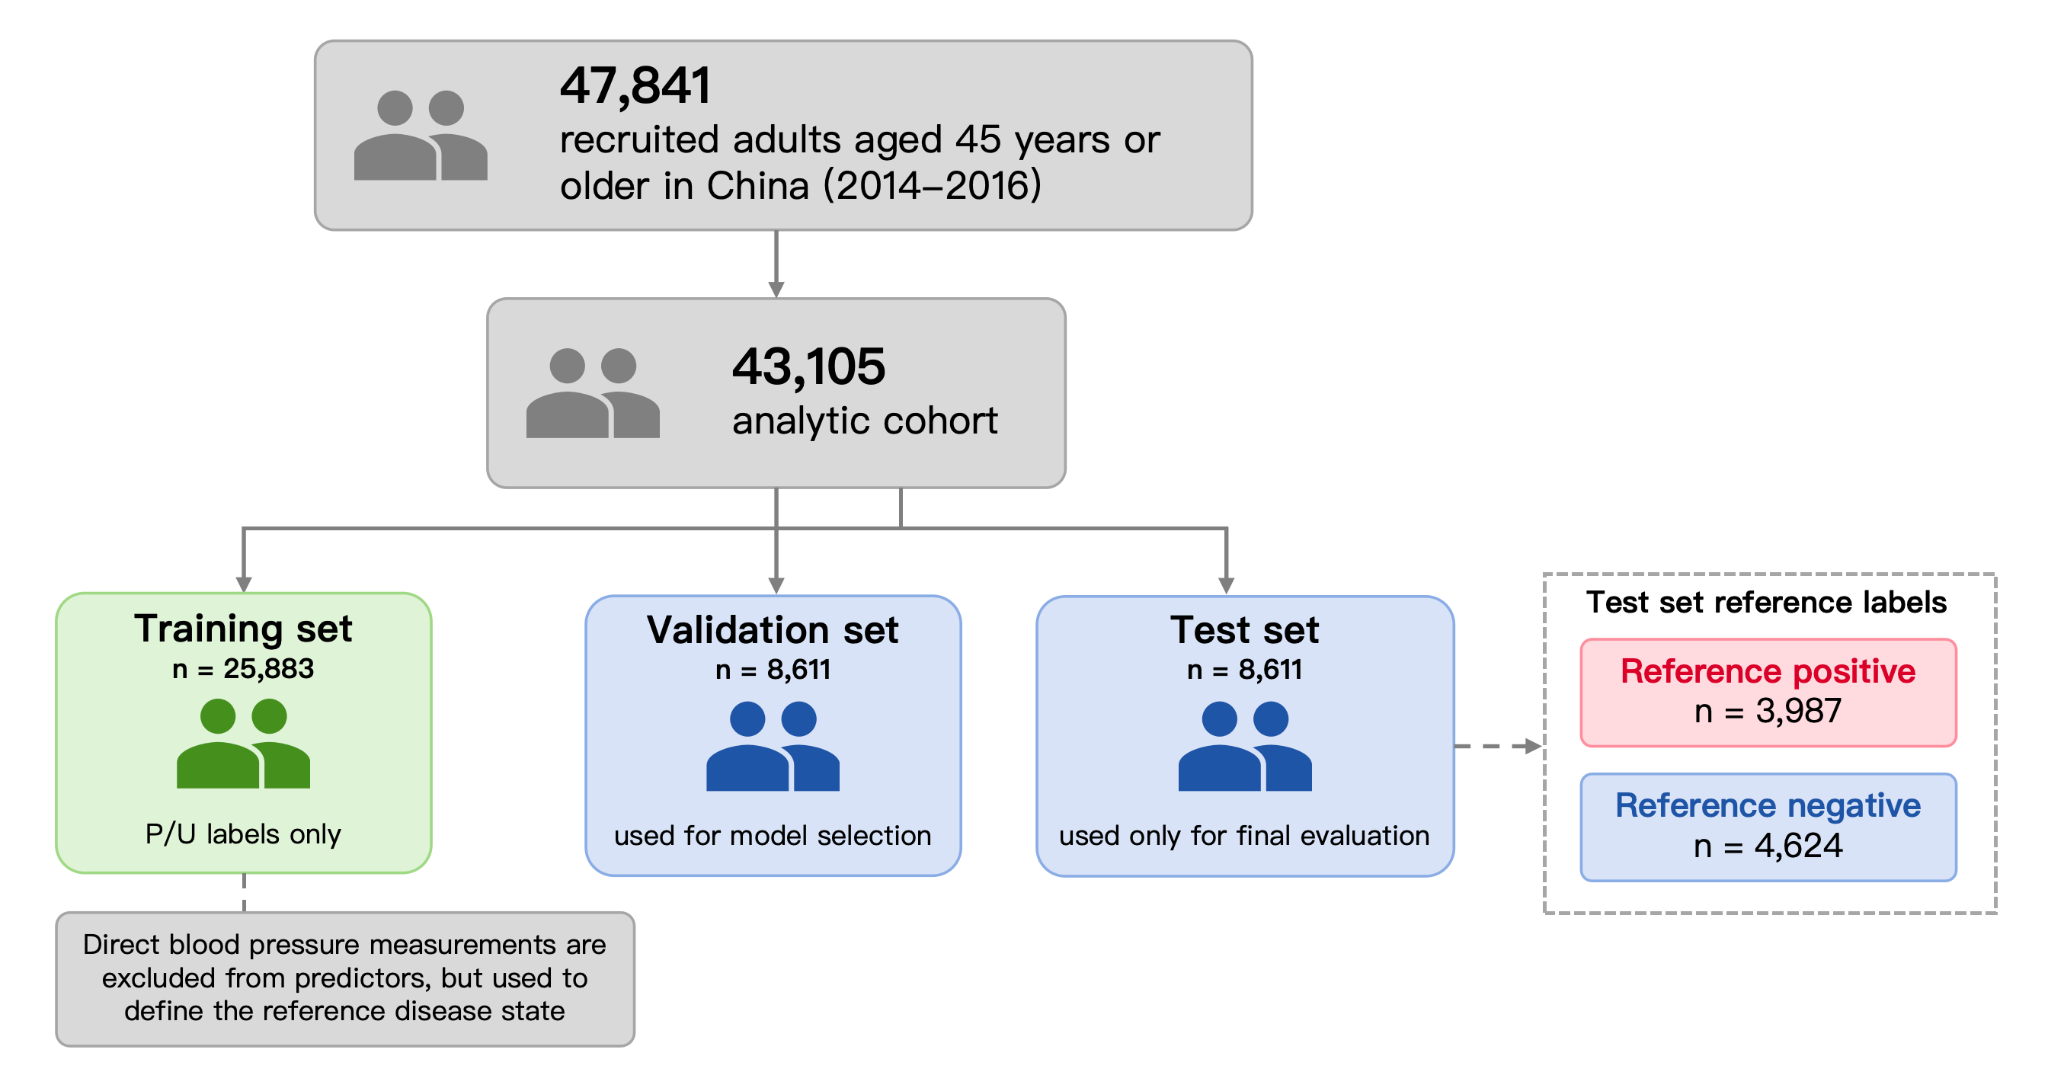
\includegraphics[width=0.92\textwidth]{figures/figure2_cohort_partition.png}
\caption{\textbf{Cohort construction, data partitioning, and information isolation.} Data collection was completed for 47,841 adults aged $\geq$45 years, Participants with missing information in variables required for model development were excluded, yielding a final analytic sample of 43,105. Participants were divided into training (n=25,883), validation (n=8,611), and test (n=8,611) sets in a 6:2:2 ratio. Two-stage PU reconstruction used only P/U information from the training set; reference disease status Y was used for validation-based model selection and final test-set evaluation. Direct blood-pressure measurements were excluded from model predictors.}
\label{fig:cohort-partition}
\end{figure*}

\subsection{Formalization of the positive-unlabeled learning
problem}\label{formalization-of-the-positive-unlabeled-learning-problem}

If the observable label \(S\) is used directly as the supervised
response, the classifier targets a quantity closer to
\(\Pr(S = 1 \mid X)\), whereas screening for undiagnosed hypertension is
concerned with \(\Pr(Y = 1 \mid X)\). Under the reliable-positive
assumption \(S = 1 \Rightarrow Y = 1\),

\[\Pr(S = 1 \mid X) = \Pr(Y = 1 \mid X)\Pr(S = 1 \mid Y = 1,X).\]

Let c(X)=Pr(S=1\textbar Y=1,X), so that
Pr(S=1\textbar X)=c(X)Pr(Y=1\textbar X). If c(X) is constant, the two
probabilities remain proportional but are generally not equal; if c(X)
varies with X, modeling the observable diagnosis label may also distort
the ordering of individual disease risk(Jain et al., 2016; Mielniczuk \&
Wawrzeńczyk, 2025). PU-Boost therefore does not interpret the stage-1
P-versus-U output as an absolute disease probability. Instead, it uses
\(P\) and \(U\) to construct a continuous screening score and
reconstructs the final supervised training set through selective
pseudo-labeling and rejection of uncertain observations.

\subsection{Assessment of distributional overlap within the unlabeled
set}\label{assessment-of-distributional-overlap-within-the-unlabeled-set}

To characterize overlap between reference-positive group B and
reference-negative group C within the unlabeled set U, exploratory
between-group analyses and low-dimensional visualizations were conducted
outside the model-training procedure using the reference labels.
Differences in the means and variances of continuous variables were
examined descriptively using two-sample t tests and F tests,
respectively. These analyses were used only to characterize task
difficulty and individual-level separability; they were not used to fit
either stage of the PU model or to construct training thresholds.

\subsection{Two-stage reliable sample
reconstruction}\label{two-stage-reliable-sample-reconstruction}

PU-Boost applies a two-stage selective pseudo-labeling procedure under
the P/U information structure. In stage 1, a regularized linear model
provides a global P-versus-U ranking and partitions the training sample
into high-confidence candidate positives, candidate negatives, and a
stage-1 uncertain set. Stage 2 refines only the uncertain set using a
nonlinear model, while observations that remain insufficiently certain
after both stages are assigned to a reject set. Rejected observations
are excluded from final binary supervised training, thereby avoiding
forced pseudo-label assignment for highly ambiguous samples.

\subsubsection{Stage 1: Global P-versus-U ranking with Elastic Net}\label{stage-1-global-p-versus-u-ranking-with-elastic-net}

Let \(X_{i} \in \mathbb{R}^{p}\) denote the feature vector for
participant \(i\). Stage 1 uses the observable training label \(S_{i}\)
as the response, coding observations in \(P\) as 1 and observations in
\(U\) as 0. Elastic Net logistic regression produces the stage-1
P-versus-U score

\[q_{i} = f_{1}\left( X_{i} \right) = \Pr\left( S_{i} = 1 \mid X_{i} \right) = \frac{1}{1 + \exp\left\lbrack - \left( \beta_{0} + X_{i}^{\mathsf{T}}\beta \right) \right\rbrack}.\]

\(q_{i}\) measures the extent to which an observation resembles the
labeled-positive set and is used for ranking and stratification(Friedman
et al., 2010; Zou \& Hastie, 2005); it is not interpreted as a
calibrated estimate of \(\Pr\left( Y_{i} = 1 \mid X_{i} \right)\).
Parameters are estimated by minimizing the penalized negative
log-likelihood:

\[
\begin{aligned}
(\widehat{\beta}_0,\widehat{\beta})
=\operatorname*{arg\,min}_{\beta_0,\beta}\Bigg\{&-\frac{1}{n}\sum_{i=1}^{n}
\Big[S_i\log q_i+(1-S_i)\log(1-q_i)\Big]\\
&+\lambda\Big[\alpha\lVert\beta\rVert_1+\frac{1-\alpha}{2}\lVert\beta\rVert_2^2\Big]\Bigg\}.
\end{aligned}
\]

where

\[\lVert\beta\rVert_1 = \sum_{j = 1}^{p}\left| \beta_{j} \right|,\quad\quad \lVert\beta\rVert_2^2 = \sum_{j = 1}^{p}\beta_{j}^{2},\]

\(\lambda\) controls the overall strength of regularization, and
\(\alpha\) controls the relative contribution of the L1 and L2
penalties; \(\alpha = 1\) corresponds to LASSO, \(\alpha = 0\)
corresponds to Ridge regression, and \(0 < \alpha < 1\) combines both
penalties. The pair \((\alpha,\lambda)\) is selected by 10-fold
cross-validation. If \(L_{k}(\alpha,\lambda)\) denotes the validation
loss in fold \(k\), then

\[CV(\alpha,\lambda) = \frac{1}{K}\sum_{k = 1}^{K}L_{k}(\alpha,\lambda),\quad\quad K = 10,\]

\[\left( \widehat{\alpha},\widehat{\lambda} \right) = \operatorname*{arg\,min}_{\alpha,\lambda}CV(\alpha,\lambda).\]

Let the stage-1 high- and low-confidence thresholds be \(t_{H}^{(1)}\)
and \(t_{L}^{(1)}\), respectively, with \(t_{L}^{(1)} < t_{H}^{(1)}\).
The stage-1 partition is defined as

\[{\widetilde{Z}}_{i}^{(1)} = \left\{ \begin{matrix}
P_{1}, & q_{i} \geq t_{H}^{(1)}, \\
N_{1}, & q_{i} \leq t_{L}^{(1)}, \\
U_{1}, & t_{L}^{(1)} < q_{i} < t_{H}^{(1)}.
\end{matrix} \right.\ \]

Here, \(P_{1}\), \(N_{1}\), and \(U_{1}\) denote the stage-1
candidate-positive set, candidate-negative set, and uncertain set,
respectively. All set memberships are determined solely from P/U
information available during training and from training-internal
threshold rules; they do not represent observed reference truth.

Specifically, the stage-1 high- and low-confidence thresholds were
defined from empirical quantiles of the P/U score distributions observed
during training. Let $Q_\gamma(\cdot)$ denote the empirical $\gamma$ quantile, and let $\alpha_1$
and $\beta_1$ denote prespecified training-stage confidence parameters:

\[t_H^{(1)} = Q_{1 - \alpha_{1}}(\{ q_{i}:\ i\  \in P\})\]

\[t_L^{(1)} = Q_{\beta_{1}}(\{ q_{i}:\ i\  \in U\})\]

Threshold construction therefore depends only on the P/U identities
available during training and their corresponding stage-1 scores $q_i$; the
reference B/C identities are not used.

\begin{figure}[!t]
\centering
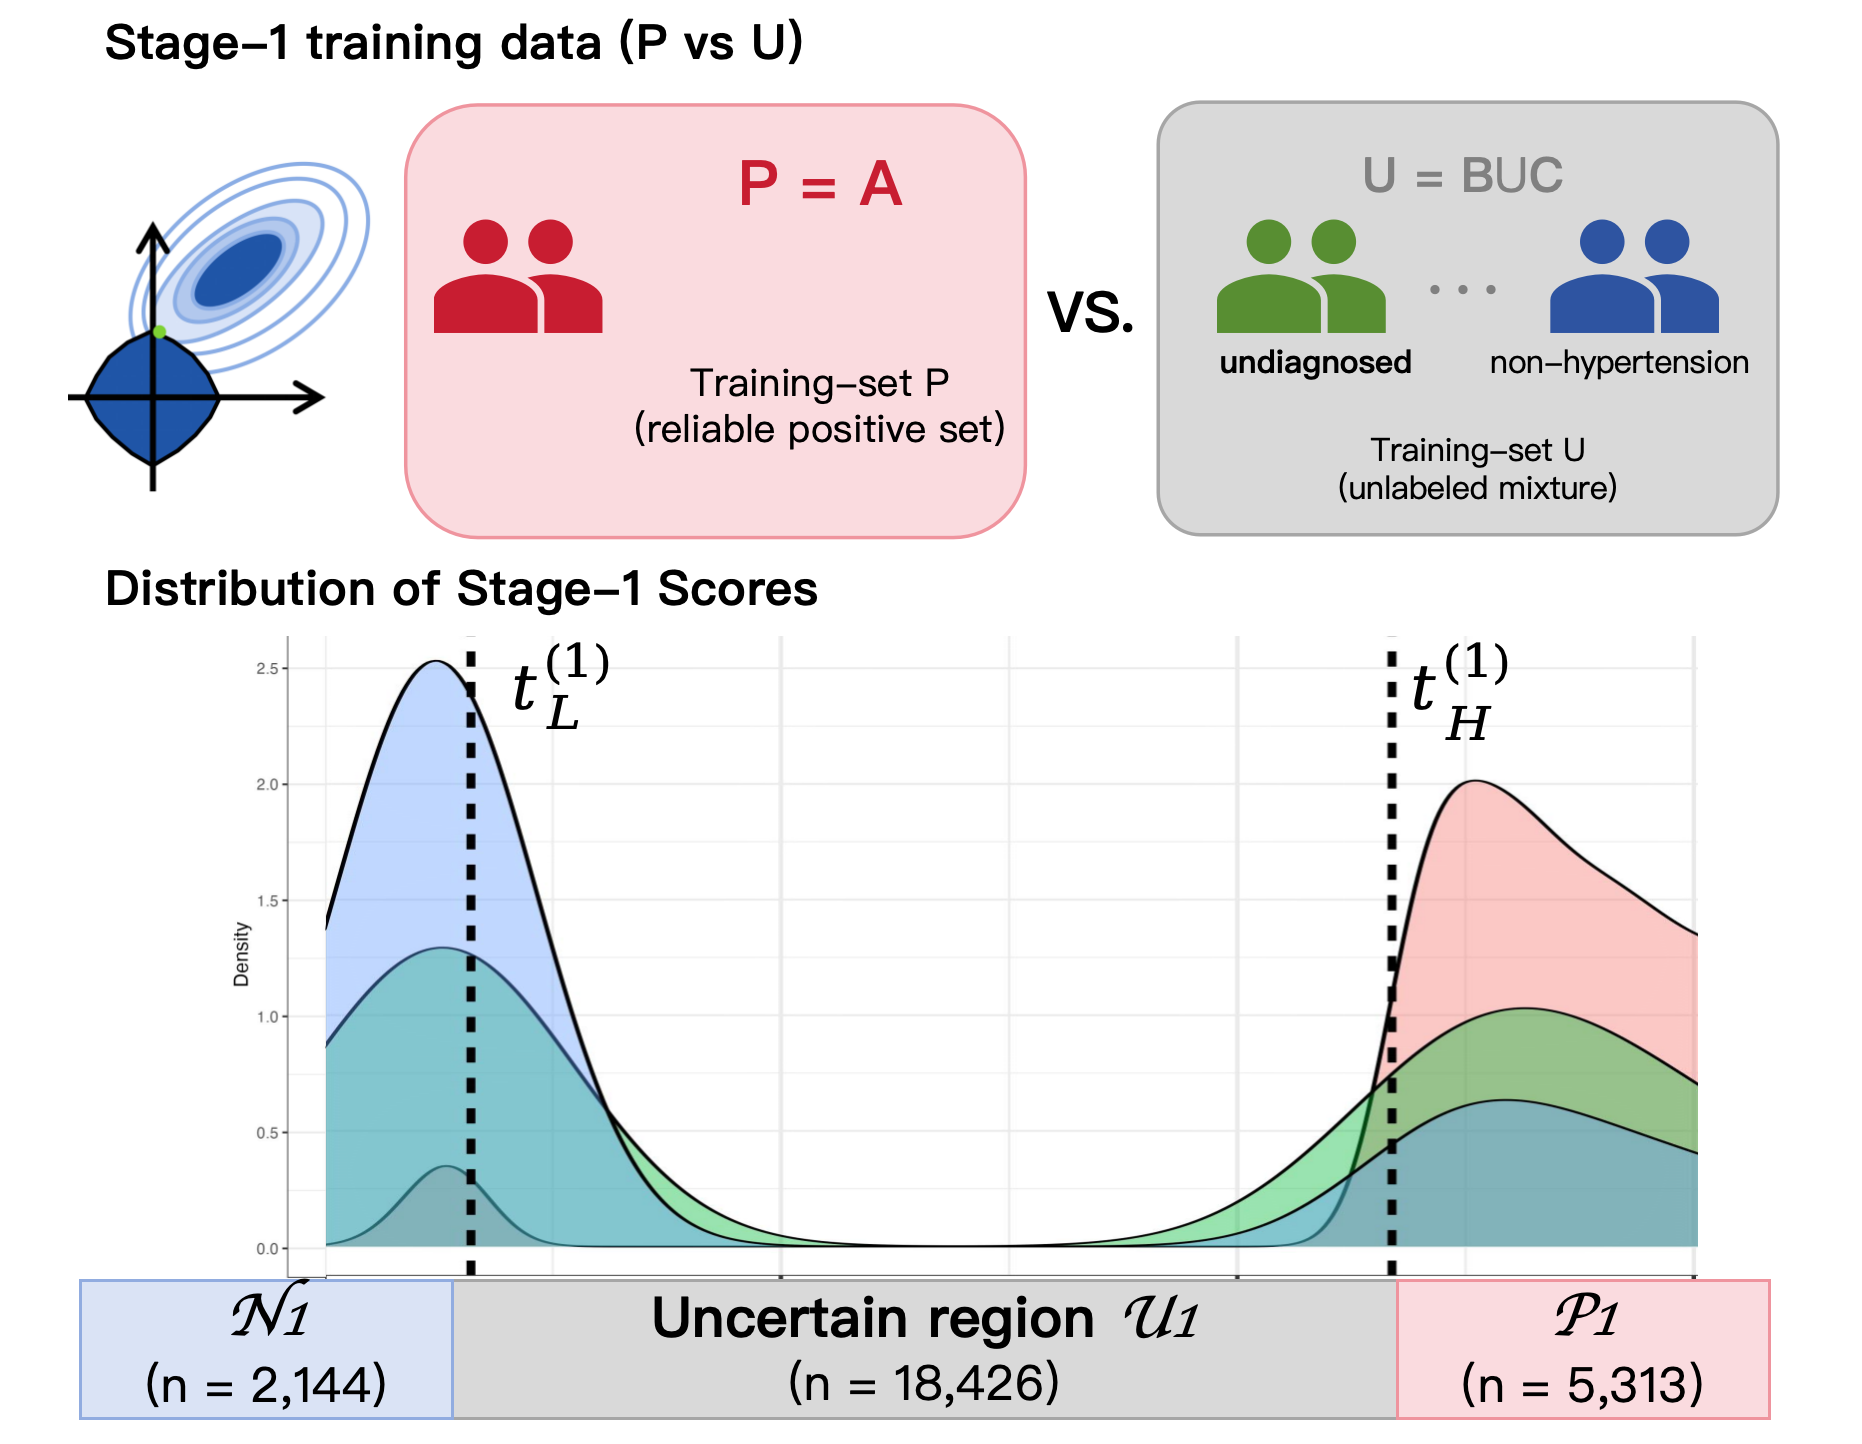
\includegraphics[width=0.98\linewidth]{figures/figure3_stage1_elasticnet.png}
\caption{\textbf{Stage-1 reliable-sample reconstruction using Elastic Net.} Elastic Net logistic regression was fitted using only training-visible P/U labels to generate the stage-1 discrimination score $q_i$. Training-internal lower and upper thresholds, $t_L^{(1)}$ and $t_H^{(1)}$, partitioned the training sample into candidate negatives $N_1$ (n=2,144), the uncertain set $U_1$ (n=18,426), and candidate positives $P_1$ (n=5,313). Reference-group score distributions, when shown, are provided only for post hoc interpretation and were not used to determine the thresholds.}
\label{fig:stage1}
\end{figure}

\subsubsection{Stage 2: Nonlinear refinement of the uncertain region using random forests}\label{stage-2-nonlinear-refinement-of-the-uncertain-region-using-random-forests}

Stage 2 is applied only to \(U_{1}\) to capture nonlinear relationships
and interactions that are not adequately represented by the stage-1
linear ranking. Let

\[r_{i} = f_{2}\left( X_{i} \right),\quad\quad i \in U_{1},\]

denote the second-stage ranking score produced by the random
forest(Breiman, 2001; Liaw \& Wiener, 2002). Let the stage-2 high- and
low-confidence thresholds be \(t_{H}^{(2)}\) and \(t_{L}^{(2)}\),
respectively, with \(t_{L}^{(2)} < t_{H}^{(2)}\). Then

\[{\widetilde{Z}}_{i}^{(2)} = \left\{ \begin{matrix}
P_{2}, & r_{i} \geq t_{H}^{(2)}, \\
N_{2}, & r_{i} \leq t_{L}^{(2)}, \\
R, & t_{L}^{(2)} < r_{i} < t_{H}^{(2)},
\end{matrix} \right.\ \quad\quad i \in U_{1}.\]

Here, \(P_{2}\) and \(N_{2}\) denote the stage-2 candidate-positive and
candidate-negative sets, respectively, and \(R\) denotes the reject set
containing observations that remain insufficiently certain after both
stages. Observations in \(R\) do not contribute to the supervised
XGBoost loss(Hendrickx et al., 2024).

The stage-2 random forest $f_2$ was trained on the supervised set formed by
the high-confidence candidates retained from stage 1. The stage-1
candidate positives $P_1$ and candidate negatives $N_1$ jointly define $D_1$ and
are assigned binary pseudo-labels $Z_i^{(1)}$=1 and $Z_i^{(1)}$=0, respectively:

\[D_{1} = P_{1} \cup N_{1}\]

\[Z_{i}^{1} = 1(i\  \in P_{1}),0(i\  \in N_{1})\]

The fitted random forest $f_2$ was then used to generate stage-2 scores $r_i$
for observations in the stage-1 uncertain set $U_1$. The high- and
low-confidence thresholds for stage 2 were defined from empirical
quantiles of the corresponding training-score distributions. Let $\alpha_2$ and
$\beta_2$ denote the stage-2 training confidence parameters:

\[t_H^{(2)} = Q_{1 - \alpha_{2}}(\{ r_{i}:\ i\  \in P_{1}\})\]

\[t_L^{(2)} = Q_{\beta_{2}}(\{ r_{i}:\ i\  \in N_{1}\})\]

Thus, both stage-2 model fitting and threshold construction rely only on
information available during training and on candidate labels generated
by stage 1; the B/C reference identities are not used.

\begin{figure}[!t]
\centering
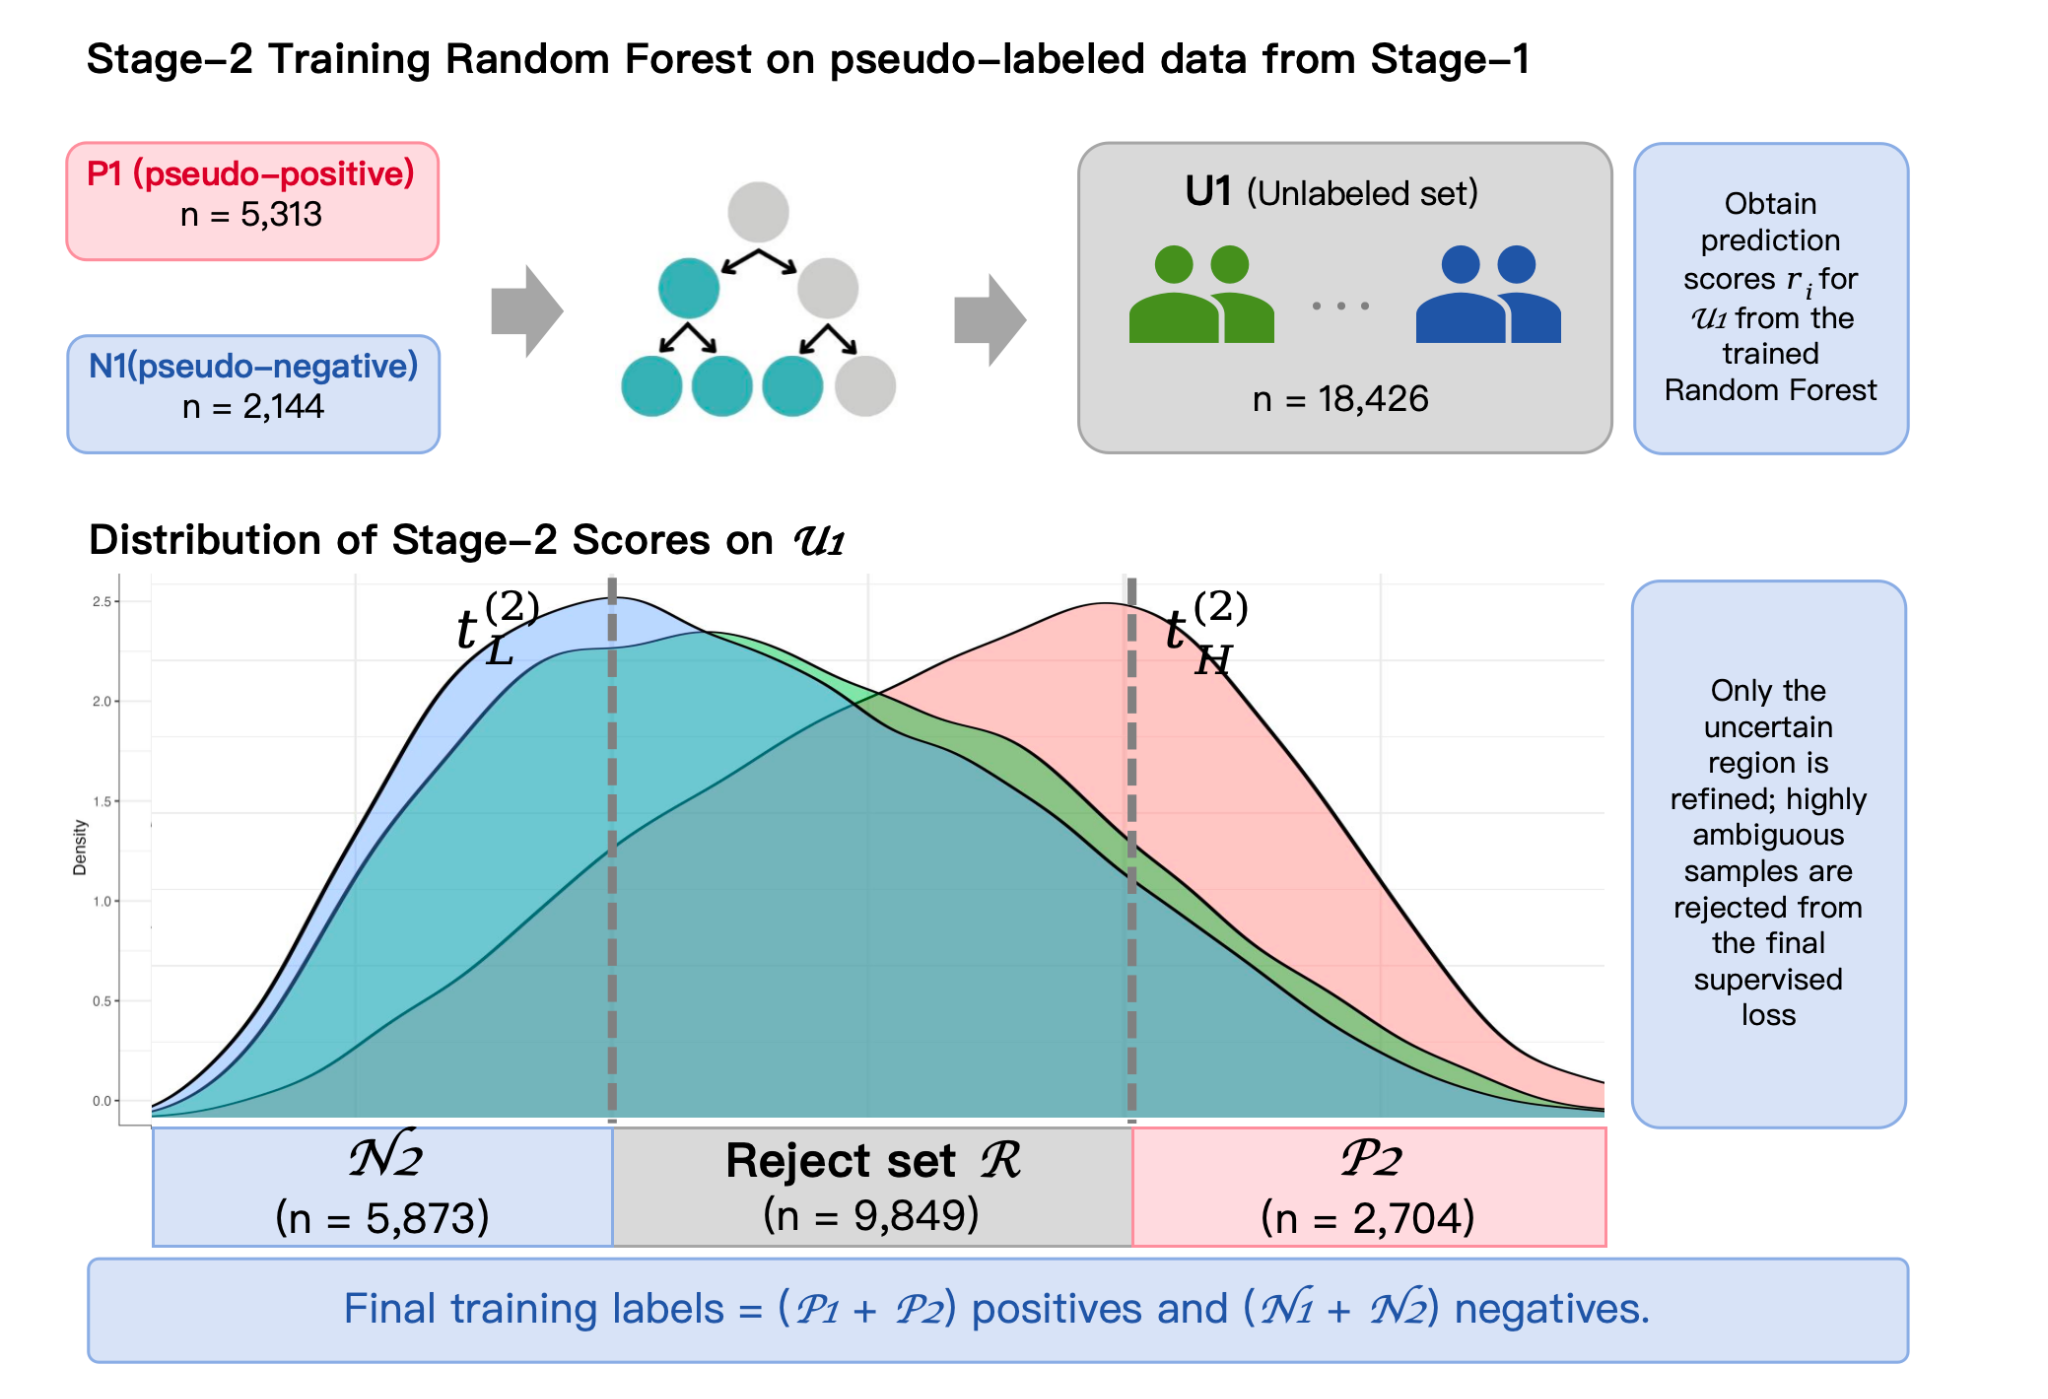
\includegraphics[width=0.98\linewidth]{figures/figure4_stage2_randomforest.png}
\caption{\textbf{Stage-2 nonlinear refinement and uncertainty rejection.} A random forest was trained using stage-1 candidate positives $P_1$ and candidate negatives $N_1$ as pseudo-labeled supervision and applied only to the uncertain set $U_1$. The resulting score $r_i$ and training-internal thresholds $t_L^{(2)}$ and $t_H^{(2)}$ partitioned $U_1$ into candidate negatives $N_2$ (n=5,873), the reject set R (n=9,849), and candidate positives $P_2$ (n=2,704). Observations in R were excluded from the final supervised loss. Reference B/C identities were not used for model fitting or threshold construction.}
\label{fig:stage2}
\end{figure}

\subsubsection{Final pseudo-labeled training set and class
balancing}\label{final-pseudo-labeled-training-set-and-class-balancing}

Candidate samples retained across the two stages were combined as

\[D_{P} = P_{1} \cup P_{2},\quad\quad D_{N} = N_{1} \cup N_{2}.\]

The final pseudo-label was defined as

\[{\widetilde{Y}}_{i} = \left\{ \begin{matrix}
1, & i \in D_{P}, \\
0, & i \in D_{N}.
\end{matrix} \right.\ \]

The final reconstructed training set contained 8,017 pseudo-positive and
8,017 pseudo-negative observations, for a total of 16,034 participants.
Because this balancing step changes the training class prior, the final
model output is interpreted primarily as a ranking and classification
score rather than as an absolute population disease probability unless
additional probability calibration is performed.

\subsection{Final classifier: XGBoost}\label{final-classifier-xgboost}

After the two-stage reconstruction, XGBoost is trained on
\(\{ X_{i},{\widetilde{Y}}_{i}\}\) to learn the final nonlinear decision
function \(g(X)\). The recorded final hyperparameters were

\[
\begin{aligned}
\text{max\_depth} &= 3, & \text{learning\_rate} &= 0.06,\\
\text{min\_child\_weight} &= 5, & \text{subsample} &= 0.5,\\
\text{colsample\_bytree} &= 0.6. &&
\end{aligned}
\]

Hyperparameters were selected by grid search using AUC with respect to
the reference disease status \(Y\) in the validation set as the
model-selection criterion(Chen \& Guestrin, 2016); the validation set
was not used in the two-stage training-sample reconstruction. The final
model produces a continuous output \({\widehat{p}}_{i}\) for each
participant. In the primary analysis, no additional probability
calibration was applied and the classification threshold was fixed at
0.5:

\[{\widehat{Y}}_{i} = \left\{ \begin{matrix}
1, & {\widehat{p}}_{i} \geq 0.5, \\
0, & {\widehat{p}}_{i} < 0.5.
\end{matrix} \right.\ \]

\subsection{Baseline models}\label{baseline-models}

To evaluate the overall effect of two-stage training-set reconstruction,
logistic regression, standard XGBoost, and a single-hidden-layer neural
network were used as baseline models. The baseline models used the same
predictors and data partition as the primary model but were trained
directly on the original observable label \(S\) and evaluated against
the reference disease status \(Y\) under the same validation/test
framework. All models were evaluated in the same test set using a
primary classification threshold of 0.5.

\subsection{Model performance
evaluation}\label{model-performance-evaluation}

Model performance was evaluated against the test-set reference disease
status \(Y\) using the confusion matrix, accuracy, sensitivity,
specificity, precision, negative predictive value, F1 score, and
balanced accuracy. Because the intended use is screening rather than
confirmatory diagnosis, particular emphasis was placed on sensitivity,
the number of false negatives, and the sensitivity-specificity
trade-off. Sensitivity and specificity were defined as

\[Sens = \frac{TP}{TP + FN},\quad\quad Spec = \frac{TN}{TN + FP}.\]

Balanced accuracy was defined as

\[BA = \frac{Sens + Spec}{2}.\]

The relative reduction in false negatives compared with a baseline model
was defined as

\[R_{FN} = \frac{FN_{baseline} - FN_{PU\text{-}Boost}}{FN_{baseline}} \times 100\%.\]

Model comparisons were descriptive. Because no paired resampling or
other formal inferential procedure was used to compare model
performance, numerical differences were not interpreted as statistically
significant.

\subsection{Model interpretation}\label{model-interpretation}

SHAP (SHapley Additive exPlanations) values were used to attribute the
final XGBoost output to individual input features(Lundberg \& Lee,
2017). SHAP summary plots were used to compare global feature
contributions, and dependence plots were used to display the direction
and potential nonlinearity of model responses for selected variables.
These analyses were used to interpret the predictive structure of the
model and were not interpreted as estimates of causal effects.

\subsection{Exploratory region-specific prevalence decision
adjustment}\label{exploratory-region-specific-prevalence-decision-adjustment}

To examine whether external region-specific hypertension prevalence
information altered the classification operating point, two exploratory
decision-adjustment strategies were evaluated. Let \({\widehat{p}}_{i}\)
denote the original PU-Boost output, \(r(i)\) denote the region of
participant \(i\), \(\pi_{r(i)}\) denote the external hypertension
prevalence for that region, and \(\pi\) denote the overall reference
prevalence(Saerens et al., 2002; Wang et al., 2018).

The first strategy adjusted model output on the logit scale:

\[s_{i}^{cal} = logit\left( {\widehat{p}}_{i} \right) + logit\left( \pi_{r(i)} \right) - logit(\pi),\]

where

\[logit(p) = log\left( \frac{p}{1 - p} \right),\]

The adjusted probability was then computed as

\[{\widehat{p}}_{i}^{cal} = \frac{1}{1 + \exp\left( - s_{i}^{cal} \right)}.\]

The second strategy directly used regional prevalence as a
region-specific classification threshold:

\[\tau_{r} = \pi_{r},\]

\[{\widehat{Y}}_{i}^{region} = \left\{ \begin{matrix}
1, & {\widehat{p}}_{i} \geq \pi_{r(i)}, \\
0, & {\widehat{p}}_{i} < \pi_{r(i)}.
\end{matrix} \right.\ \]

Both adjustments were evaluated in the same test set used for the
primary analysis. They were intended to characterize how external
prevalence priors shift the sensitivity-specificity operating point,
rather than to demonstrate an improvement in the intrinsic
discriminative ability of the model.

\subsection{Software and
reproducibility}\label{software-and-reproducibility}

All data processing, statistical analyses, model fitting, performance
evaluation, and visualization were conducted in R version 4.6.0(R Core
Team, 2025). Elastic Net logistic regression was implemented with the
glmnet package(Friedman et al., 2010), random forests with
randomForest(Liaw \& Wiener, 2002), gradient boosting with xgboost(Chen
\& Guestrin, 2016), and the single-hidden-layer neural network with
nnet. ROC/AUC calculations were performed using pROC. SHAP values for
the final XGBoost model were computed with fastshap and summarized and
visualized with shapviz(Greenwell, 2024). Random seeds were fixed for
cross-validation, random-forest fitting, negative-class downsampling,
and other stochastic procedures to improve reproducibility. The
principal analysis code, model implementation, and scripts required to
reproduce the main results are available in a public GitHub repository
at
\href{https://github.com/LionelWu11282562/A-Two-Stage-Probability-Stratified-Method-for-Ambiguous-Dataset-Optimization}{{[}GitHub
repository URL{]}}. Package versions and complete
computational-environment information are also recorded in the
repository.

\section{Results}

\subsection{Cohort composition and label structure}

A total of 43,105 participants were included. Based on prior diagnosis
and reference disease status, participants were retrospectively
classified into three groups: diagnosed hypertension (group A; n=13,287,
30.8\%), undiagnosed hypertension (group B; n=9,393, 21.8\%), and
non-hypertensive individuals (group C; n=20,425, 47.4\%). The A/B/C
grouping was used to describe the reference disease structure of the
cohort and for downstream model selection and performance evaluation.
During two-stage PU reconstruction, only group A served as the
labeled-positive set P; the reference identities of groups B and C were
hidden from the training algorithm and together formed the unlabeled set
U.

The data were split in a 6:2:2 ratio into training, validation, and test
sets containing 25,883, 8,611, and 8,611 participants, respectively. The
test set contained 3,987 reference-positive and 4,624 reference-negative
participants. Model fitting preserved the P/U information structure,
while the reference disease status was used only in the corresponding
model-selection and performance-evaluation stages.

\begin{table*}[!t]
\caption{\textbf{Reference-group composition and label structure of the analytic cohort.} Group membership was defined retrospectively from prior hypertension diagnosis and reference blood-pressure status. During PU reconstruction, group A constituted the labeled-positive set P, whereas groups B and C jointly constituted the unlabeled set U. Percentages are based on the full analytic cohort (N=43,105).}
\label{tab:cohort}
\centering
\small
\setlength{\tabcolsep}{7.5pt}
\renewcommand{\arraystretch}{1.08}
\begin{tabular}{@{}clrrrrl@{}}
\toprule
\textbf{Reference group} & \textbf{Clinical definition} & \textbf{n} & \textbf{\%} & \textbf{$Y$} & \textbf{$S$} & \textbf{PU role} \\
\midrule
A & Diagnosed hypertension & 13,287 & 30.8 & 1 & 1 & Labeled positive P \\
B & Undiagnosed hypertension & 9,393 & 21.8 & 1 & 0 & Unlabeled U \\
C & Non-hypertensive & 20,425 & 47.4 & 0 & 0 & Unlabeled U \\
Total & --- & 43,105 & 100.0 & --- & --- & --- \\
\bottomrule
\end{tabular}
\end{table*}

\textbf{Distributional overlap and label uncertainty within the
unlabeled population}

Exploratory group-level analyses indicated distributional differences
among groups A, B, and C across multiple demographic, behavioral,
medical-history, and anthropometric variables. However, these
group-level differences did not translate into clear individual-level
separation. Low-dimensional representations and score distributions
showed substantial overlap between group B and group C in the available
feature space.

These findings indicate substantial sample-level uncertainty between
reference-positive and reference-negative observations within U, making
the two components difficult to separate reliably using a single simple
decision boundary. Accordingly, subsequent modeling focused on
progressively identifying observations with higher label confidence
while preventing highly uncertain observations from being forced into
the final supervised training set.

\begin{figure}[!t]
\centering
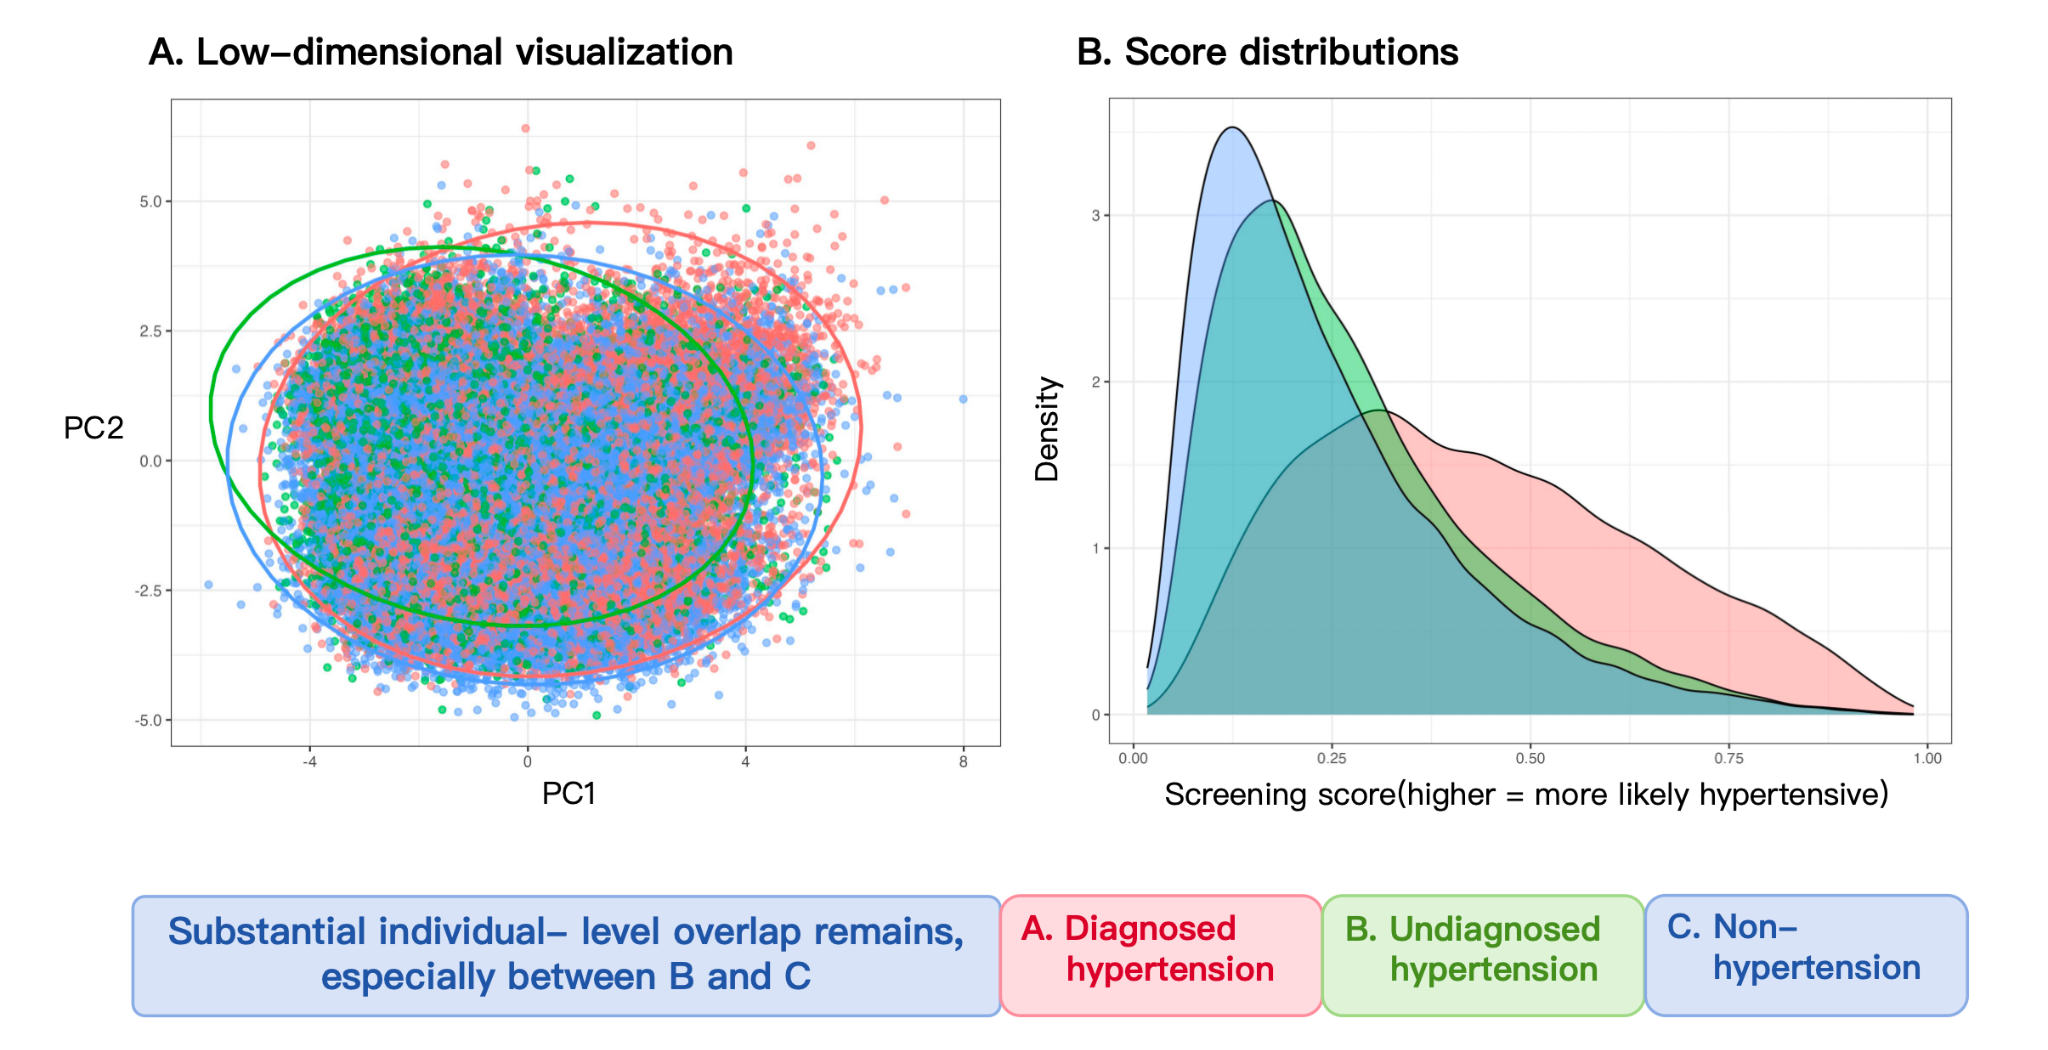
\includegraphics[width=0.98\linewidth]{figures/figure5_distribution_overlap.png}
\caption{\textbf{Distributional overlap among reference groups in the available predictor space.} (A) Principal-component representation of diagnosed hypertension (A), undiagnosed hypertension (B), and non-hypertensive participants (C). (B) Distribution of the stage-1 P-versus-U score stratified retrospectively by reference group. Substantial individual-level overlap remained, particularly between groups B and C. Reference group identities are displayed for post hoc interpretation only and were not used during PU reconstruction.}
\label{fig:overlap}
\end{figure}

\subsection{Two-stage pseudo-label reconstruction}

The training set was first scored by Elastic Net logistic regression for
global P-versus-U stratification. Under the prespecified stage-1
training thresholds, the 25,883 training observations were partitioned
into 5,313 candidate positives, 2,144 candidate negatives, and 18,426
observations in the uncertain set $U_1$. Thus, under the prespecified
confidence thresholds, 18,426 participants (71.2\%) were retained in $U_1$
for stage-2 nonlinear refinement.

Stage 2 applied a random forest only to $U_1$. The 18,426 uncertain
observations were further partitioned into 2,704 stage-2 candidate
positives, 5,873 candidate negatives, and 9,849 highly ambiguous
observations. The highly ambiguous subset was excluded from final
classifier training, implementing a reject option for observations that
remained insufficiently certain after both stages.

After combining candidates retained across both stages, the
reconstructed training set contained 8,017 pseudo-positive and 8,017
pseudo-negative observations, for a total of 16,034 participants (61.9\%
of the original training set); the remaining 9,849 highly uncertain
observations (38.1\%) were excluded. The resulting class-balanced
training sample was therefore composed of candidates retained at high
confidence across the two reconstruction stages, while highly uncertain
observations did not contribute directly to the final empirical loss.

\begin{figure*}[!t]
\centering
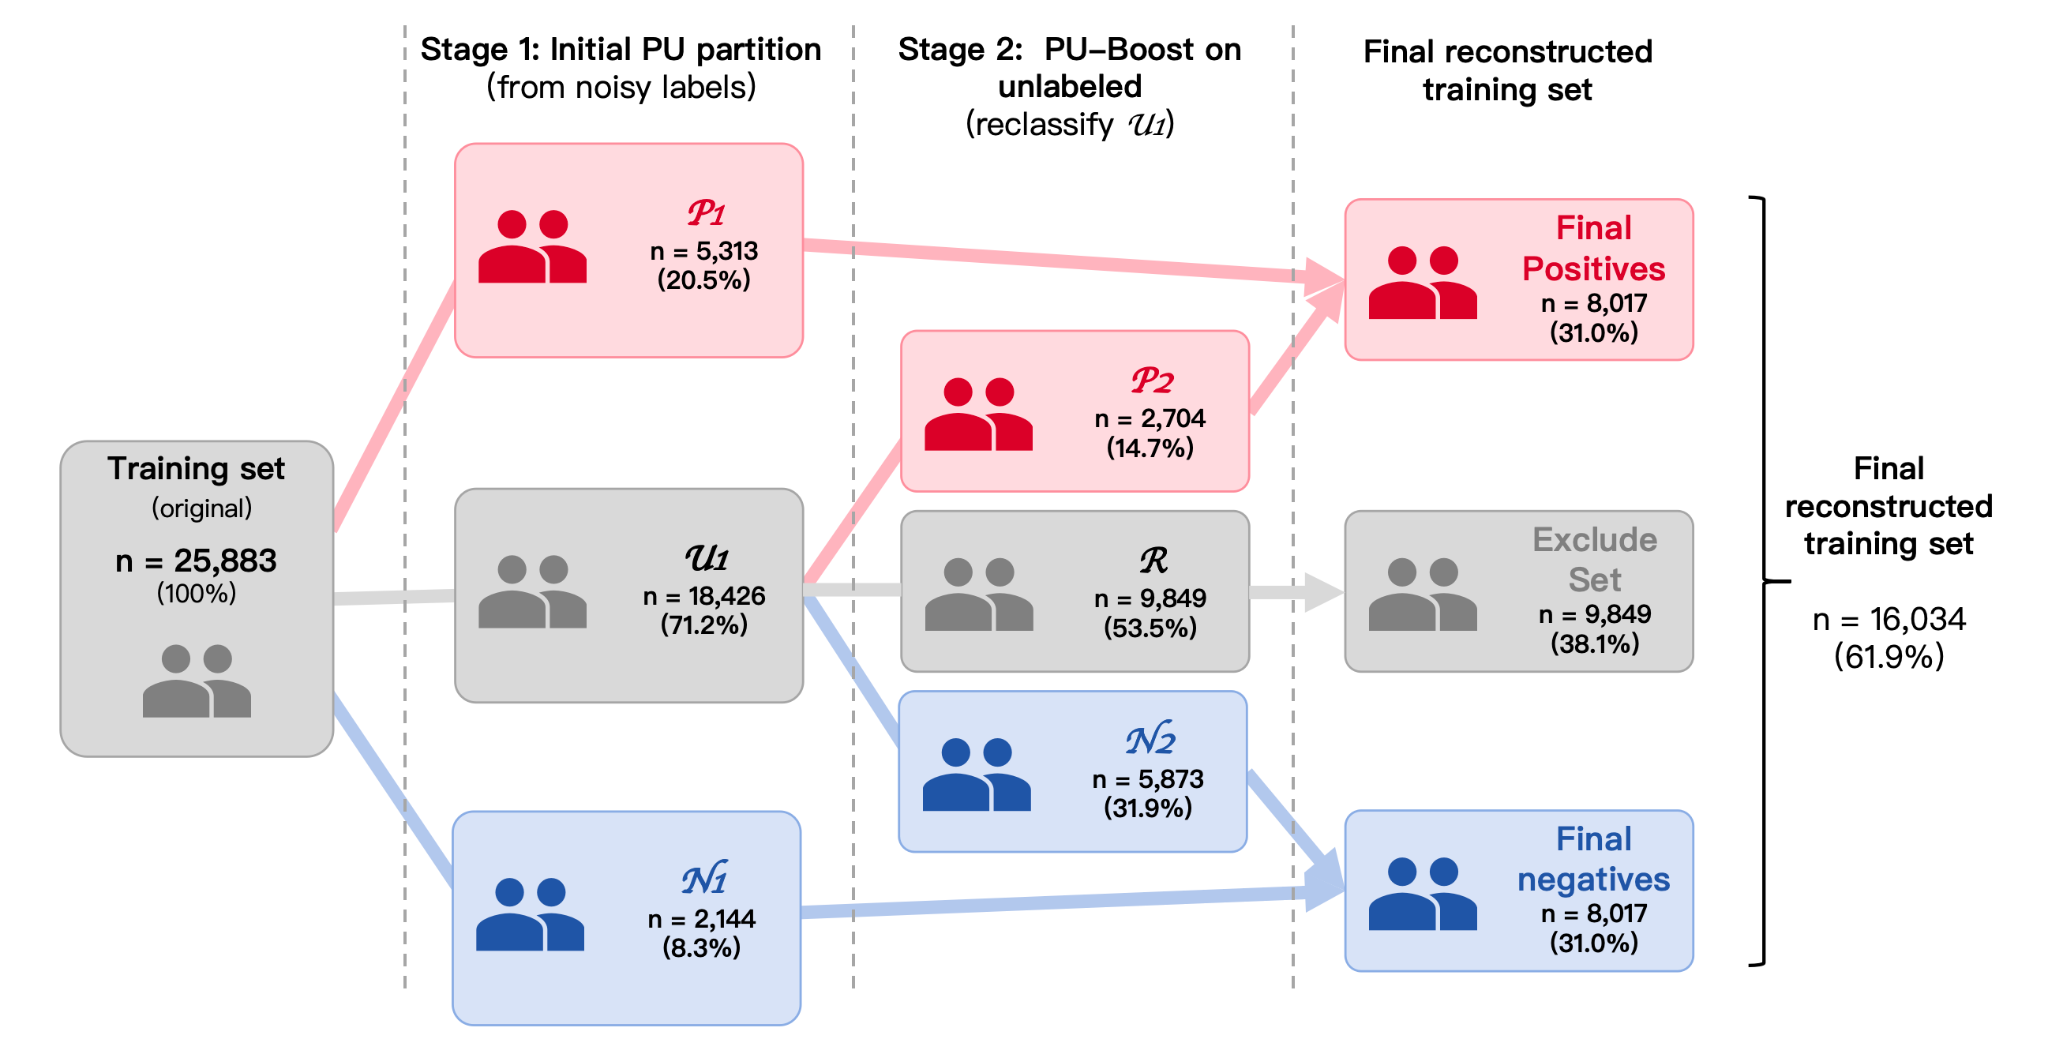
\includegraphics[width=0.95\textwidth]{figures/figure6_reconstruction_flow.png}
\caption{\textbf{Sample flow through the two-stage reliable-sample reconstruction procedure.} The original training set (n=25,883) was partitioned at stage 1 into $P_1$ (n=5,313), $N_1$ (n=2,144), and $U_1$ (n=18,426). Stage 2 further divided $U_1$ into $P_2$ (n=2,704), $N_2$ (n=5,873), and the reject set R (n=9,849). Combining retained candidates yielded 8,017 pseudo-positive and 8,017 pseudo-negative observations, forming a final reconstructed training set of 16,034 participants (61.9\% of the original training set); 9,849 observations (38.1\%) were rejected.}
\label{fig:reconstruction-flow}
\end{figure*}

\subsection{Predictive performance comparison}

PU-Boost was compared with three conventional supervised-learning
models: logistic regression, standard XGBoost, and a neural network. At
the prespecified classification threshold of 0.5, PU-Boost achieved a
sensitivity of 0.8172 in the test set, the highest observed value among
the compared models, versus 0.6832 for logistic regression, 0.6897 for
standard XGBoost, and 0.7186 for the neural network. Relative to
standard XGBoost, sensitivity increased by 0.1275 in absolute terms.

PU-Boost achieved a balanced accuracy of 0.6823, also the highest
observed value, compared with 0.6624 for logistic regression, 0.6618 for
standard XGBoost, and 0.6382 for the neural network. Overall accuracy
was 0.6723 and likewise exceeded that of the three baselines. In
contrast, the specificity of PU-Boost was 0.5474, lower than that of
logistic regression and standard XGBoost.

The principal performance advantage of PU-Boost was therefore higher
positive-case detection and balanced accuracy rather than uniform
improvement across all classification metrics. Its test-set behavior
reflected a high-sensitivity operating point, with improved
identification of reference-positive cases at the cost of lower
specificity.

\begin{table*}[!t]
\caption{\textbf{Test-set predictive performance of PU-Boost and baseline models.} All models were evaluated against the reference disease status Y in the same independent test set (n=8,611) using a classification threshold of 0.5. TP, true positives; TN, true negatives; FP, false positives; FN, false negatives; NPV, negative predictive value. Boldface indicates the highest observed value for each performance metric. Model comparisons are descriptive.}
\label{tab:performance}
\centering
\setlength{\tabcolsep}{3.8pt}
\renewcommand{\arraystretch}{1.08}
\resizebox{\textwidth}{!}{%
\begin{tabular}{@{}lrrrrrrrrrrr@{}}
\toprule
\textbf{Model} & \textbf{TP} & \textbf{TN} & \textbf{FP} & \textbf{FN} & \textbf{Accuracy} & \textbf{Sensitivity} & \textbf{Specificity} & \textbf{Precision} & \textbf{NPV} & \textbf{F1} & \textbf{Balanced Accuracy} \\
\midrule
Logistic Regression & 2724 & 2967 & 1657 & 1263 & 0.6609 & 0.6832 & \textbf{0.6417} & \textbf{0.6218} & 0.7014 & 0.6511 & 0.6624 \\
XGBoost & 2750 & 2931 & 1693 & 1237 & 0.6597 & 0.6897 & 0.6339 & 0.6190 & 0.7032 & 0.6524 & 0.6618 \\
Neural Network & 2865 & 2579 & 2045 & 1122 & 0.6322 & 0.7186 & 0.5577 & 0.5835 & 0.6968 & 0.6440 & 0.6382 \\
PU Boost & 3258 & 2531 & 2093 & 729 & \textbf{0.6723} & \textbf{0.8172} & 0.5474 & 0.6089 & \textbf{0.7764} & \textbf{0.6978} & \textbf{0.6823} \\
\bottomrule
\end{tabular}}
\end{table*}

\subsection{Reduction in missed cases and screening-oriented performance}

PU-Boost produced 729 false negatives in the test set, the fewest among
the compared models. Logistic regression, standard XGBoost, and the
neural network produced 1,263, 1,237, and 1,122 false negatives,
respectively. The corresponding reductions in false negatives with
PU-Boost were 42.3\%, 41.1\%, and 35.0\%.

Compared with standard XGBoost, PU-Boost reduced the number of false
negatives from 1,237 to 729, corresponding to 508 additional
reference-positive participants being identified. This gain was
accompanied by more false positives and lower specificity, indicating
that the principal change was a redistribution of error types rather
than a cost-free improvement in all aspects of classification
performance.

This operating point is aligned with a screening objective that
prioritizes reduction of missed cases: reference-positive individuals
are more likely to be flagged for follow-up, while false-positive
high-risk classifications can subsequently be resolved by standard
blood-pressure measurement. PU-Boost is therefore better positioned as a
high-sensitivity risk-stratification tool before confirmatory
measurement than as a substitute for definitive clinical diagnosis.

\begin{figure*}[!t]
\centering
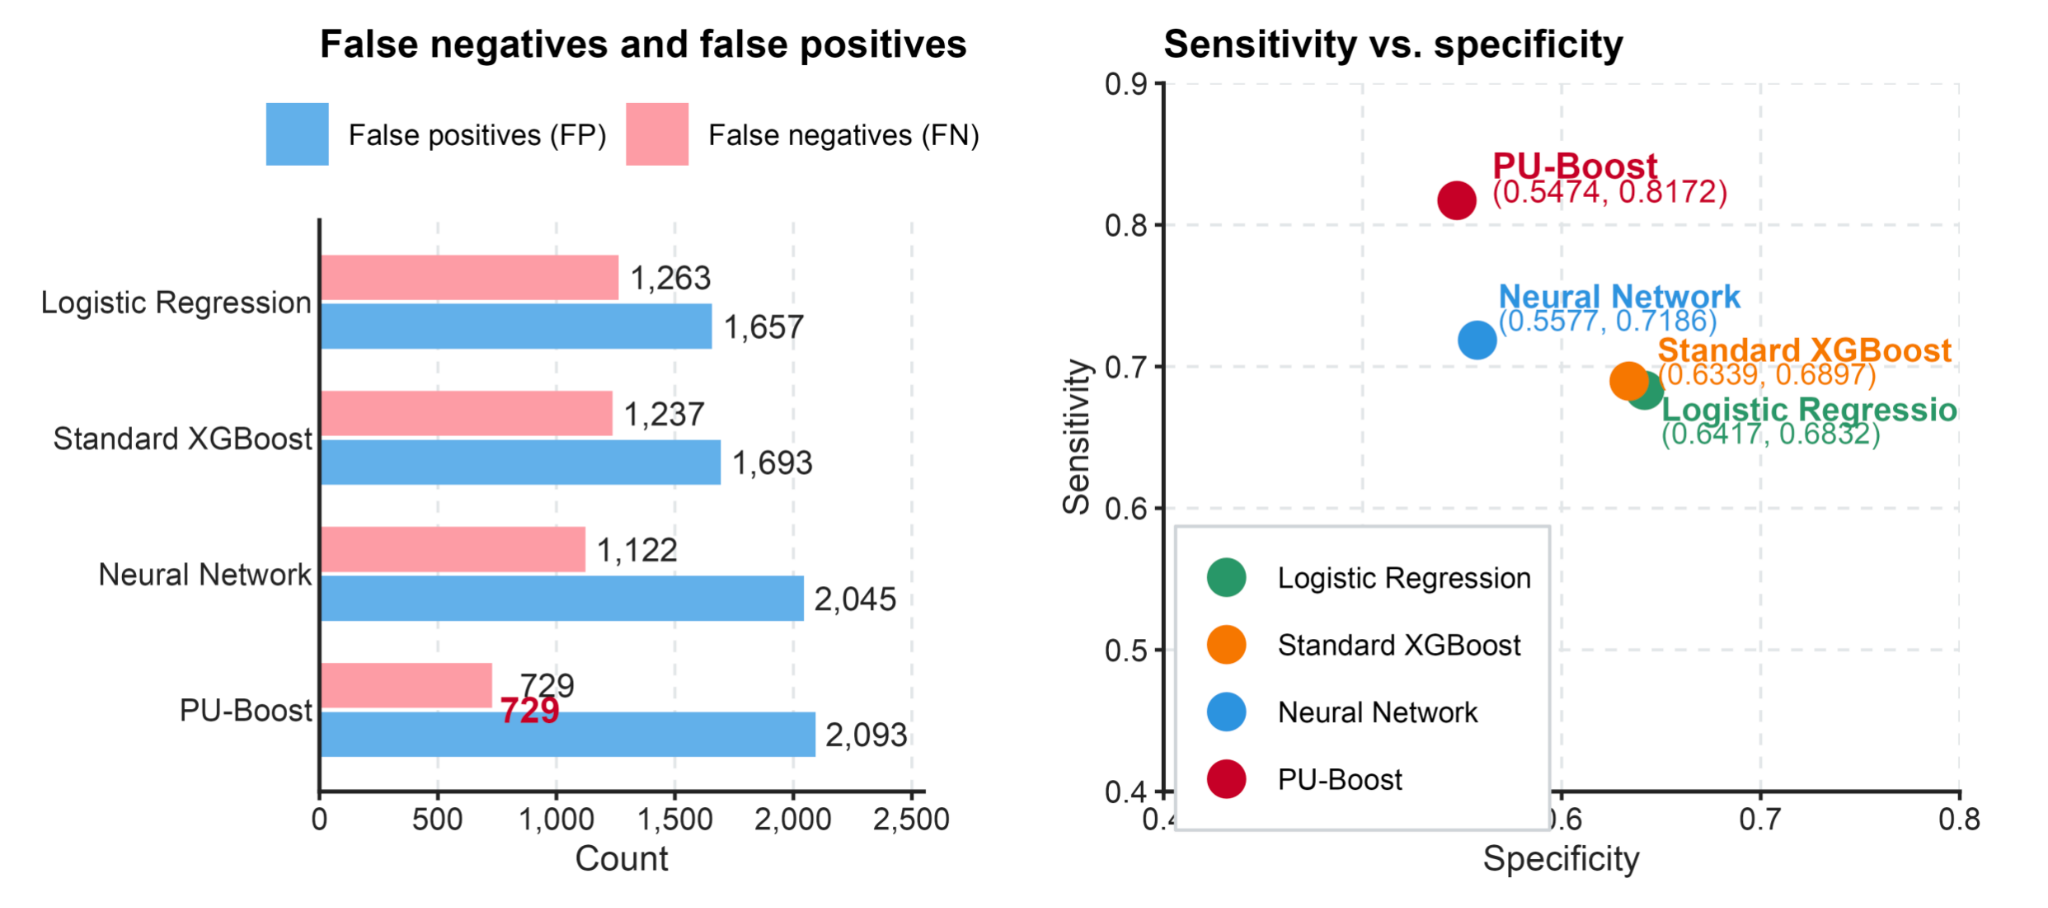
\includegraphics[width=0.91\textwidth]{figures/figure7_performance.png}
\caption{\textbf{Test-set predictive performance and error profiles of PU-Boost and baseline models.} (A) Sensitivity-specificity operating points at the prespecified classification threshold of 0.5. (B) Numbers of false negatives and false positives for logistic regression, standard XGBoost, the neural network, and PU-Boost. PU-Boost achieved the highest observed sensitivity and the fewest false negatives, accompanied by a higher number of false positives and lower specificity.}
\label{fig:performance}
\end{figure*}

\subsection{Feature-importance analysis}

SHAP analysis was used to quantify the contribution of each input
feature to the final PU-Boost output. Age had the largest global SHAP
contribution, followed by body mass index (BMI) and waist circumference.
Other features among the ten highest-ranked global contributors included
maternal history of hypertension, paternal history of hypertension,
snoring, dyslipidemia, history of stroke, current smoking, and diabetes.

These highly ranked features are broadly consistent with established
epidemiologic knowledge of hypertension and include age, general and
central adiposity, family history, sleep-related factors, and metabolic
and cardiovascular history. This concordance suggests that the final
model relied substantially on clinically interpretable predictors,
although SHAP values describe model attribution and do not establish
causal effects or pathophysiologic mechanisms.

In addition to conventional risk-related variables, indicators for
Xinjiang, Jiangxi, and Guangdong showed relatively large SHAP
contributions, indicating that geographic information contributed to
prediction. These contributions may reflect regional differences in
exposure profiles, lifestyle, socioeconomic conditions, or access to
health care, but the underlying mechanisms cannot be determined from
SHAP analysis alone.

Overall, the major predictive contributions in PU-Boost were
concentrated in variables with recognizable clinical and epidemiologic
interpretations, providing feature-level insight into the model output.

\begin{figure*}[!t]
\centering
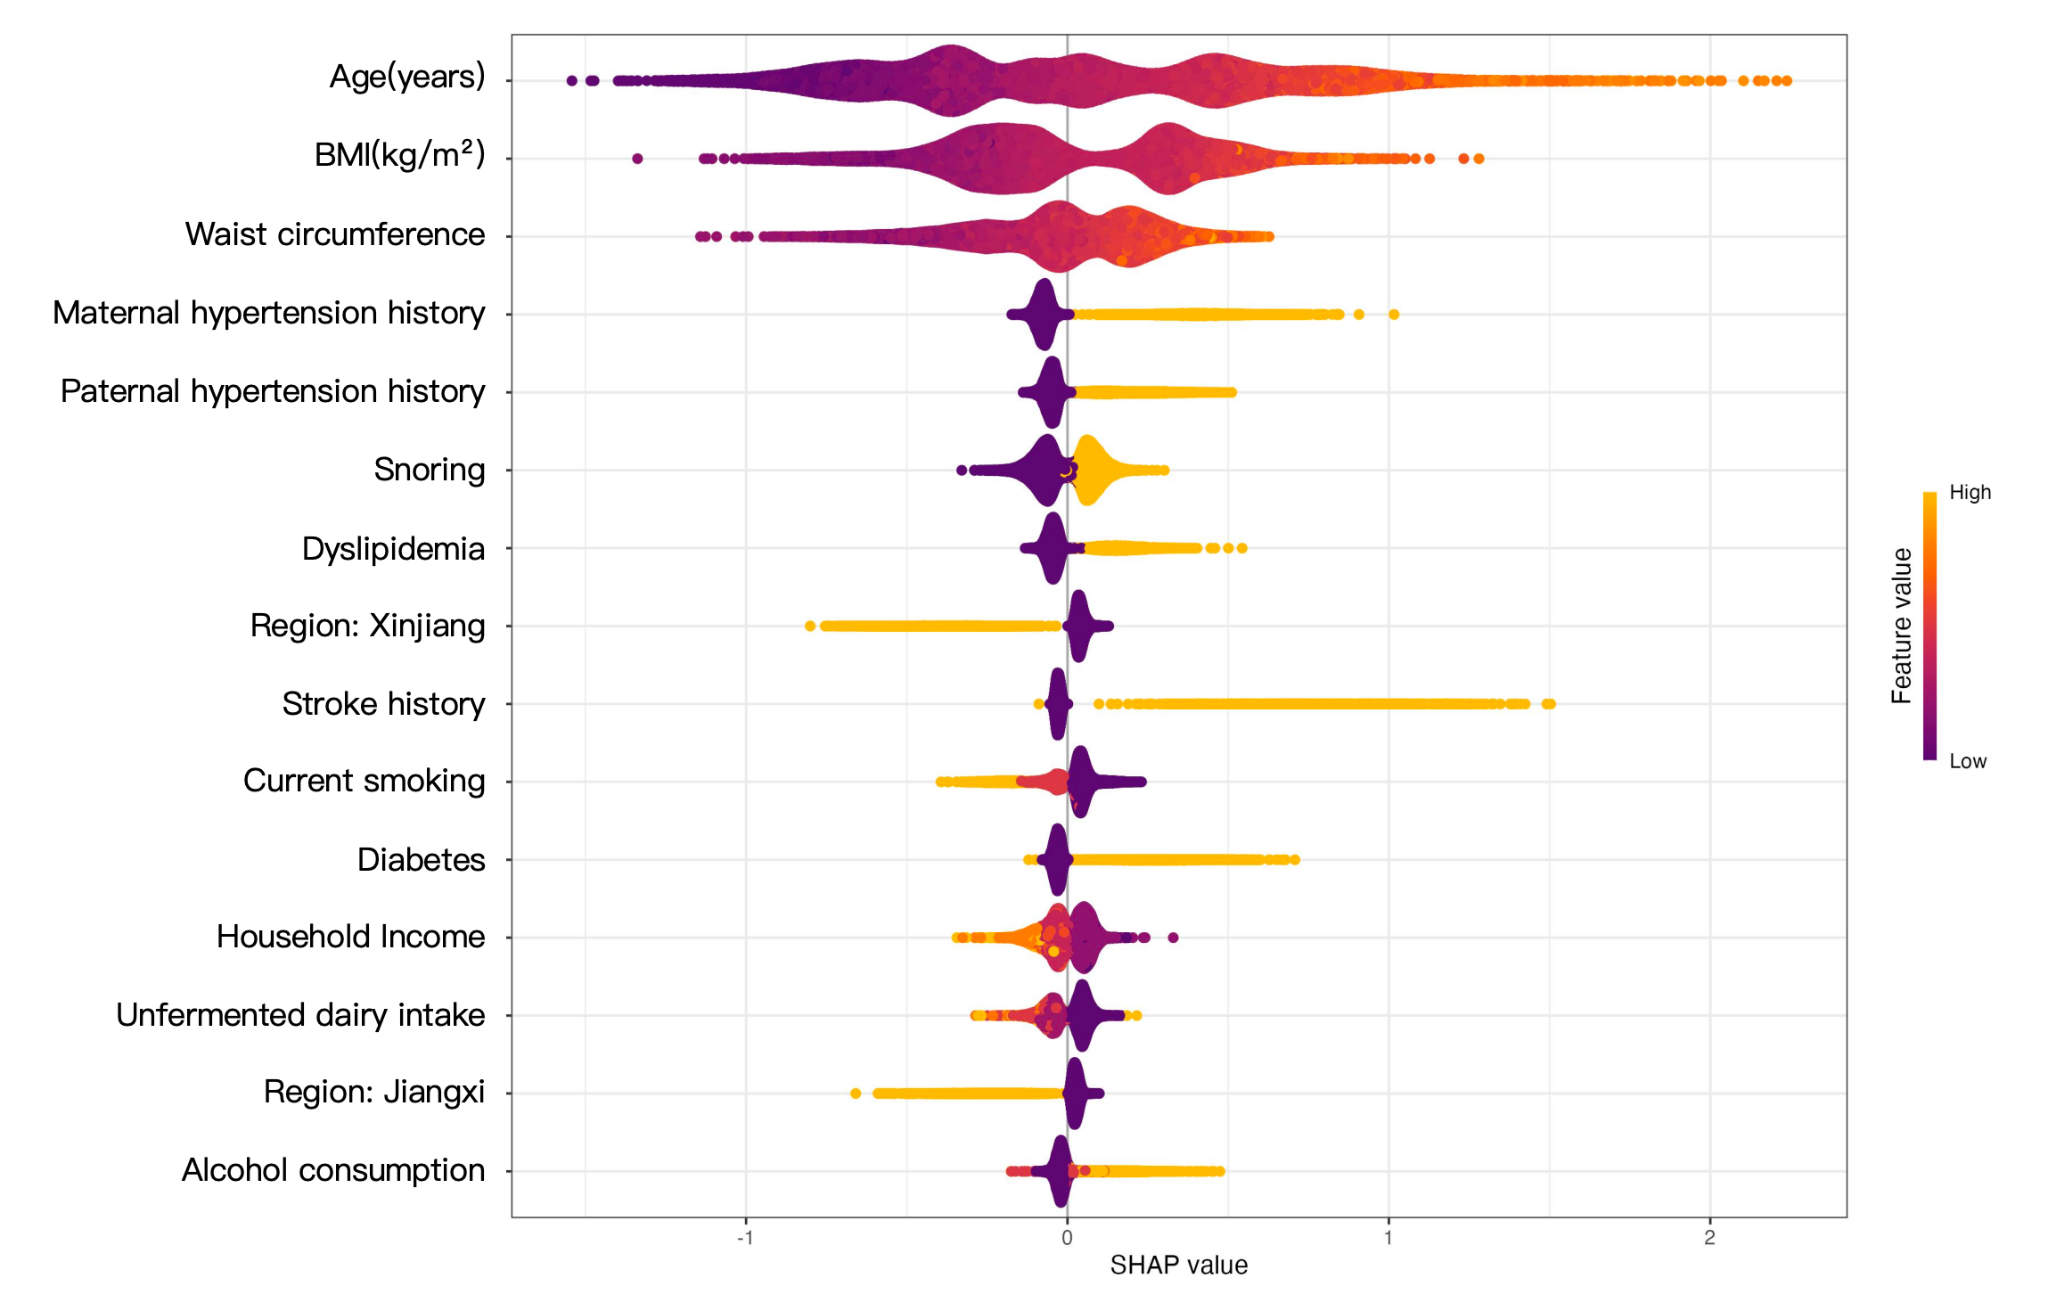
\includegraphics[height=2.30in]{figures/figure8a_shap_summary.png}\hspace{0.18in}%
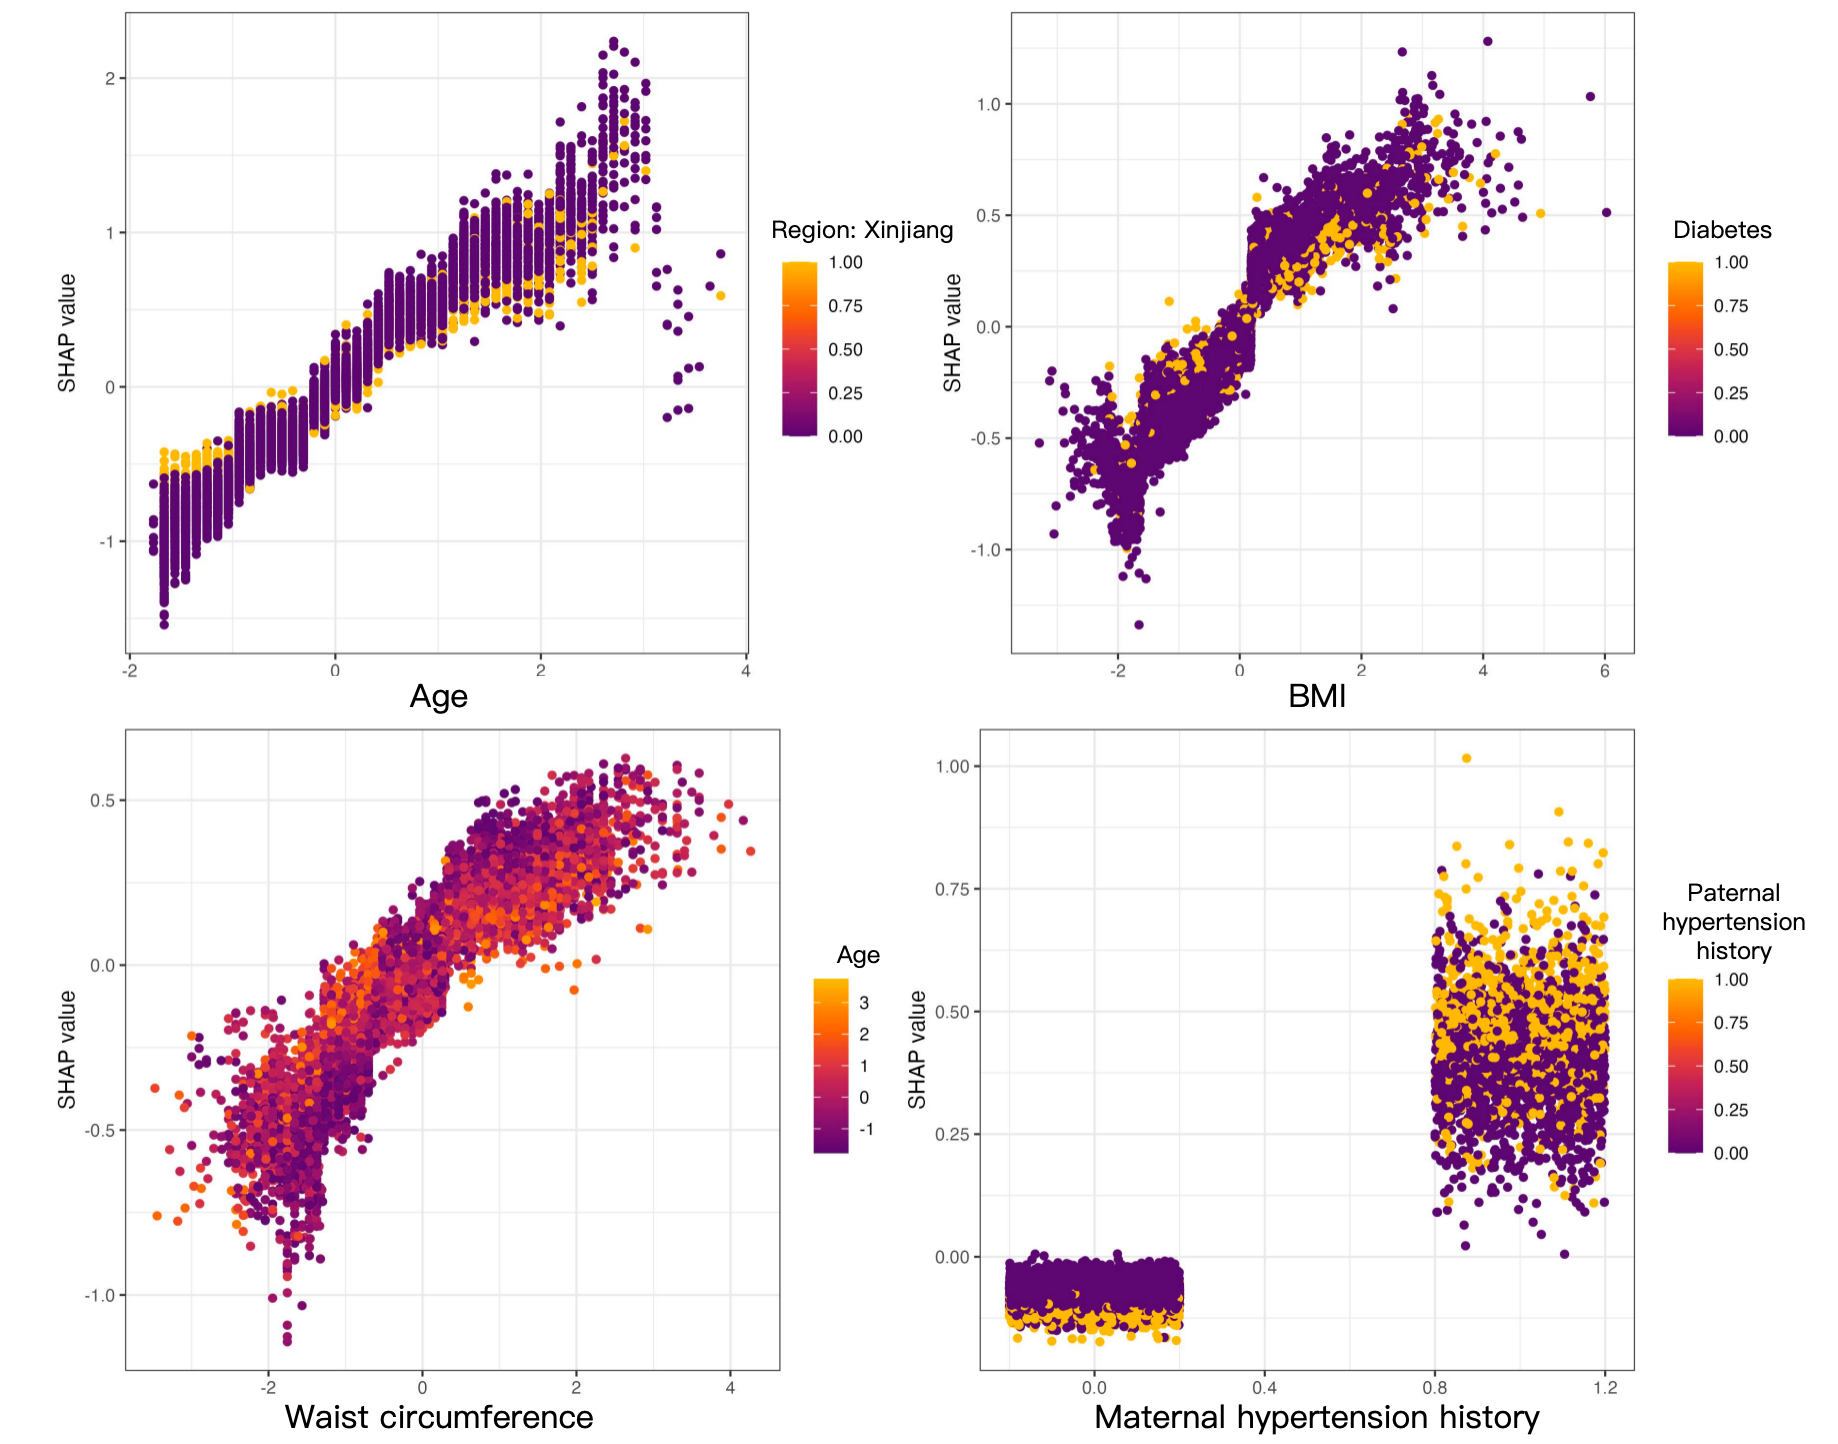
\includegraphics[height=2.30in]{figures/figure8b_shap_dependence.png}
\caption{\textbf{SHAP-based interpretation of the final PU-Boost model.} (A) SHAP beeswarm plot showing the leading global contributors to model output, ordered by mean absolute SHAP value. Higher and lower feature values are indicated by the color scale. (B--E) SHAP dependence plots for age, body mass index, waist circumference, and maternal history of hypertension; color denotes the indicated secondary feature. SHAP values represent model attribution and should not be interpreted as causal effects.}
\label{fig:shap}
\end{figure*}

\subsection{Exploratory region-specific prevalence decision adjustment}\label{exploratory-region-specific-prevalence-decision-adjustment-results}

As an exploratory analysis, we examined whether external region-specific
hypertension prevalence information altered the operating point of
PU-Boost. The unadjusted PU-Boost model had a sensitivity of 0.817,
specificity of 0.547, F1 score of 0.698, and balanced accuracy of 0.682.

The region-logit adjustment increased specificity to 0.885 but reduced
sensitivity to 0.369; the corresponding F1 score and balanced accuracy
were 0.491 and 0.627. The region-specific prevalence-threshold
adjustment produced similar results, with specificity of 0.871,
sensitivity of 0.398, F1 score of 0.514, and balanced accuracy of 0.634.

Relative to the original operating point, the region-logit adjustment
increased specificity by 0.338 while reducing sensitivity by 0.448. The
prevalence-threshold adjustment increased specificity by 0.324 while
reducing sensitivity by 0.419. Neither strategy improved the F1 score or
balanced accuracy.

Thus, external regional prevalence information primarily shifted the
sensitivity-specificity trade-off rather than improving overall
screening performance under the metrics considered here. For a screening
setting in which reduction of false negatives is prioritized, the
original PU-Boost operating point retained substantially higher
positive-case detection.

\begin{table*}[!t]
\caption{\textbf{Test-set performance under the original and region-specific decision rules.} The original PU-Boost operating point was compared with region-logit and region-prevalence threshold adjustments using the same test-set predictions. Regional adjustments were exploratory and were intended to modify the sensitivity-specificity operating point rather than to improve the intrinsic discrimination of the fitted model.}
\label{tab:region-adjustment}
\centering
\small
\setlength{\tabcolsep}{8pt}
\renewcommand{\arraystretch}{1.08}
\begin{tabularx}{\textwidth}{@{}Xccccc@{}}
\toprule
\textbf{Method} & \textbf{Sensitivity} & \textbf{Specificity} & \textbf{Precision} & \textbf{F1} & \textbf{Balanced Accuracy} \\
\midrule
PU Boost & \textbf{0.817} & 0.547 & 0.609 & 0.698 & \textbf{0.682} \\
Region-logit adjustment & 0.369 & \textbf{0.885} & 0.735 & 0.491 & 0.627 \\
Region-prevalence threshold adjustment & 0.398 & \textbf{0.871} & 0.727 & 0.514 & 0.634 \\
\bottomrule
\end{tabularx}
\end{table*}

\begin{figure}[!t]
\centering
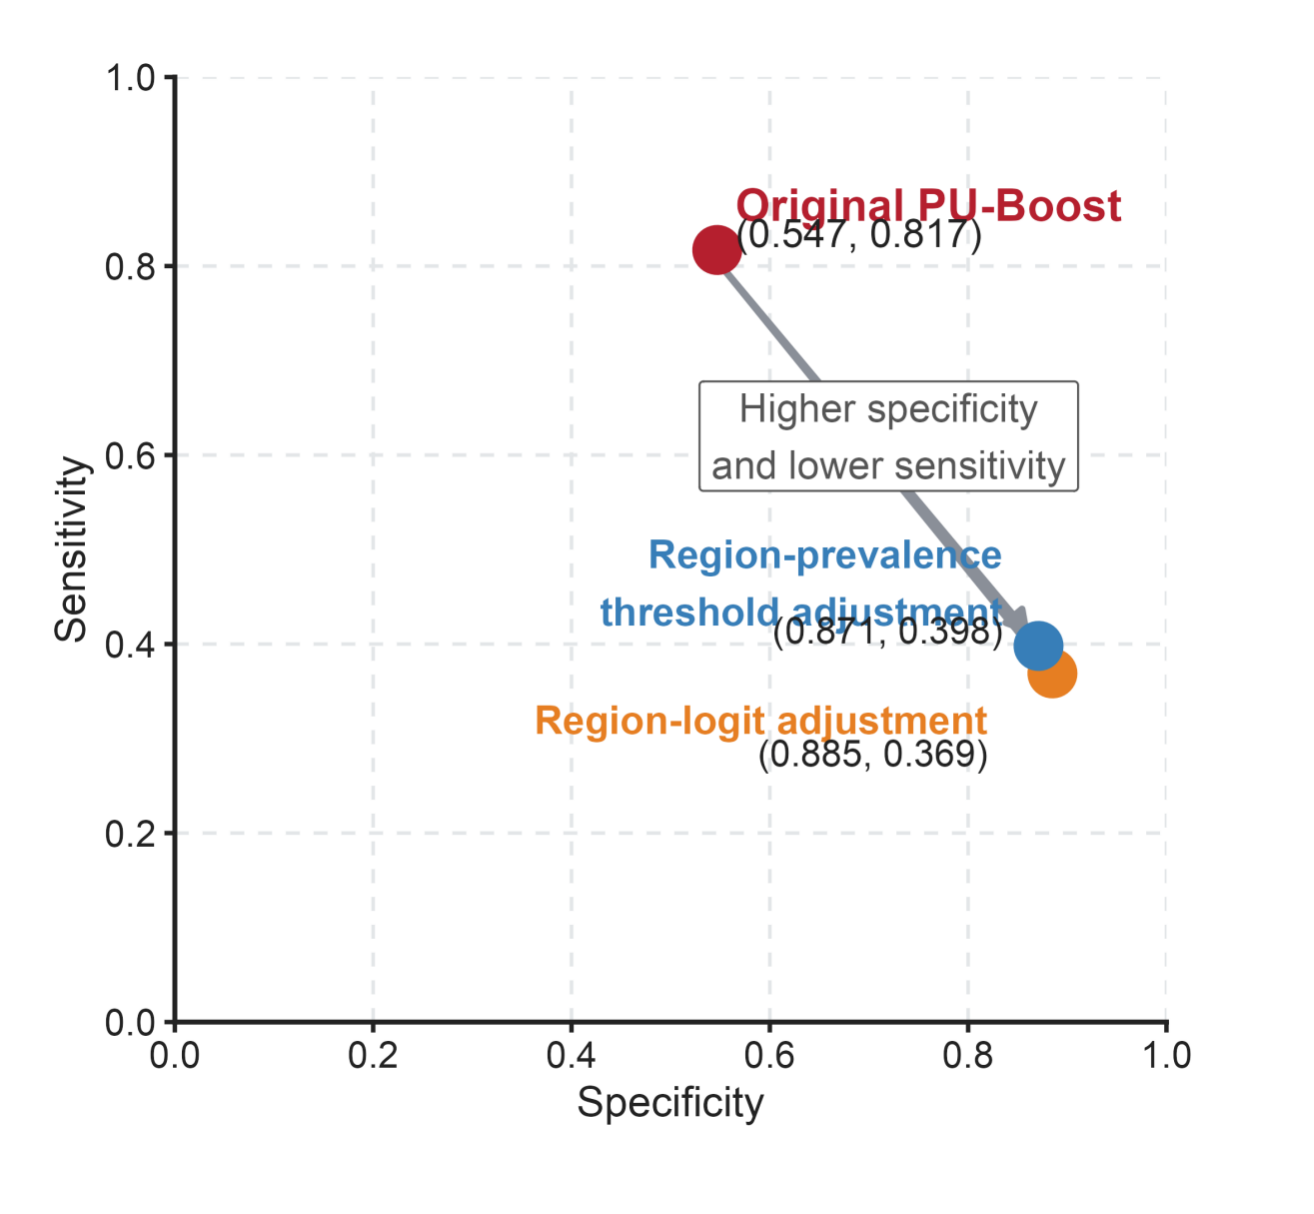
\includegraphics[width=0.95\linewidth]{figures/figure9_region_adjustment.png}
\caption{\textbf{Sensitivity-specificity operating points under exploratory region-specific decision adjustments.} The original PU-Boost operating point is compared with region-logit and region-prevalence threshold adjustments in the same test set. Both regional adjustments shifted the operating point toward higher specificity and substantially lower sensitivity, indicating a change in the decision rule rather than an improvement in intrinsic model discrimination.}
\label{fig:region-adjustment}
\end{figure}

\section{Discussion}

This study formulates screening for undiagnosed hypertension as a
positive-unlabeled learning problem and introduces PU-Boost, a two-stage
reliable-sample reconstruction framework. The central issue is the
mismatch between the observable diagnosis label and the reference
disease status: training observes only labeled positives $P=A$ and the
unlabeled set $U=B\cup C$, while U contains both hidden reference-positive and
reference-negative individuals. A supervised classifier trained directly
on S minimizes empirical risk with respect to the observable label,
whereas the screening target is defined by Y(Bekker \& Davis, 2020;
Elkan \& Noto, 2008); probabilistically, the corresponding targets are
Pr(S=1\textbar X) and Pr(Y=1\textbar X). The methodological motivation
for PU-Boost is therefore not to increase classifier complexity per se,
but to reconstruct the training supervision so that hidden positives do
not systematically contribute negative labels to the final classifier.

The two-stage architecture of PU-Boost can be interpreted as regularized
global ranking, local nonlinear refinement, and rejection of
persistently uncertain observations(Bekker \& Davis, 2020; Hendrickx et
al., 2024; Liu et al., 2002). Elastic Net extracts stable global
discrimination from the P/U label structure and separates readily
classifiable observations from an uncertain region. A random forest is
then applied only to this uncertain region to exploit nonlinear
relationships and interactions. Observations that remain insufficiently
certain after both stages are not forced into binary pseudo-labels but
are excluded from final classifier training. The procedure therefore
trades sample size for reduced direct contribution of highly uncertain
supervision to the final empirical loss. Its potential benefit should be
attributed to the joint reconstruction of the training distribution and
supervision rather than to a simple sequence of Elastic Net, random
forest, and XGBoost classifiers.

The independent test-set results were consistent with the intended
screening behavior of this reconstruction strategy. At the prespecified
threshold, PU-Boost achieved a sensitivity of 0.8172 and balanced
accuracy of 0.6823, both the highest observed values among the compared
models. Relative to standard XGBoost, sensitivity increased by 0.1275
and false negatives decreased from 1,237 to 729, a reduction of 508
cases (41.1\%). These findings indicate that, for the same prediction
task, PU-Boost tended to recover more reference-positive individuals
missed by the conventional supervised baseline. However, the results
support the overall two-stage reconstruction pipeline and do not
establish that the performance difference arose solely from more
accurate pseudo-labels. PU-Boost simultaneously modifies sample
selection, the training class ratio, and the final operating point;
without component-specific ablation analyses, their individual
contributions cannot be separately quantified.

The most prominent change in error structure was a shift from false
negatives toward false positives. PU-Boost produced fewer false
negatives than the baseline models but had a specificity of 0.5474 and
generated more false positives. Thus, the method did not improve every
evaluation dimension simultaneously; rather, it operated at a more
sensitivity-oriented screening point. From a decision perspective, this
operating point is consistent with a screening context in which false
negatives carry a higher relative cost. For hypertension screening, a
false negative corresponds to a participant with reference hypertension
being classified as low risk and potentially remaining unidentified,
whereas a false positive can be reassessed by standard blood-pressure
measurement. When the cost of missing disease exceeds the cost of
additional confirmation, this error allocation may have practical
screening value. Conversely, the lower specificity would be a
substantial limitation if the model were used for definitive diagnosis.
PU-Boost should therefore be viewed as a pre-confirmatory
risk-stratification tool rather than a replacement for clinical
diagnosis.

SHAP analysis provided further insight into the predictive structure of
the final model. Age, BMI, waist circumference, parental history of
hypertension, snoring, dyslipidemia, diabetes, history of stroke, and
smoking contributed strongly to model output and are broadly consistent
with established epidemiologic knowledge of hypertension(Herzog et al.,
2025; Kolifarhood et al., 2019; Oparil et al., 2018; Peppard, 2000; Su
et al., 2024). Several regional indicators also had relatively large
SHAP contributions, suggesting that geographic information contributed
to prediction, potentially through differences in exposure patterns,
lifestyle, socioeconomic conditions, or health-care access(Zhou et al.,
2019). Because SHAP quantifies attribution to model output rather than
causal effects, these findings support clinical interpretability of the
predictive structure but do not establish pathophysiologic mechanisms or
exclude reliance on proxy variables or noise.

The exploratory prevalence-based decision adjustments further
demonstrate the dependence of classification performance on the selected
operating rule. Both the region-logit and region-specific threshold
adjustments increased specificity but substantially reduced sensitivity
and lowered both F1 score and balanced accuracy. External prevalence
information therefore shifted the sensitivity-specificity operating
point without improving discrimination under the metrics used
here(Saerens et al., 2002; Wang et al., 2018). In other words, the
threshold is a deployment-level decision parameter rather than an
intrinsic property of discrimination; the same continuous score can map
to different false-negative/false-positive trade-offs under different
thresholds. For the present screening objective, which prioritizes
reduction of missed cases, the unadjusted operating point was more
consistent with the intended application.

Several limitations should be considered. First, PU learning assumes
that labeled positives are sufficiently reliable, yet the process
determining whether a hypertensive individual has been previously
diagnosed is unlikely to be random. The labeling mechanism
Pr(S=1\textbar Y=1,X) may vary with health-care access, health
awareness, geography, socioeconomic status, and other covariates,
producing positive-selection bias(Chang et al., 2022; Jain et al., 2016;
Mielniczuk \& Wawrzeńczyk, 2025). Second, two-stage sample selection,
rejection of uncertain observations, and 1:1 class balancing jointly
alter the composition and class prior of the training set, so the
observed increase in sensitivity cannot be attributed uniquely to any
single component(du Plessis et al., 2015; du Plessis et al., 2014; Kiryo
et al., 2017; Li et al., 2022; Wu et al., 2023). Third, to preserve a
simple screening setting, laboratory measurements, medication
information, and direct blood-pressure measurements were intentionally
excluded from predictors. This improves feasibility of data collection
but may limit the achievable predictive performance. Fourth, the
relatively low specificity of PU-Boost may increase false-positive
volume and confirmatory workload in large-scale deployment, and its net
practical value will depend on the screening cost structure. Fifth, the
study population comprised community-dwelling adults aged $\geq$45 years from
eight study areas in China. The findings should not be directly
extrapolated to younger populations or other settings, and external
validation in additional datasets is needed to establish
transportability.

Future work should prioritize three directions. First, the sensitivity,
false-negative reduction, and specificity of PU-Boost should be
evaluated in independent external datasets to assess the stability of
the training-sample reconstruction strategy. Second, the framework
should be compared systematically with alternative PU-learning,
weak-supervision, and mixture-model approaches, with component-specific
analyses used where feasible to separate the effects of sample
selection, class balancing, and uncertainty rejection. Third, decision
thresholds should be optimized with respect to the relative costs of
missed cases, confirmatory blood-pressure measurement, and acceptable
false-positive burden in the intended screening workflow. Only after low
false-negative rates and manageable confirmation burden are demonstrated
externally should broader application to other screening problems with a
reliable-positive plus mixed-unlabeled structure be considered.

\section{Conclusion}

We developed PU-Boost, a two-stage reliable-sample reconstruction
positive-unlabeled learning framework for screening undiagnosed
hypertension. Under a label structure consisting of reliable positives
and a mixed unlabeled population, PU-Boost progressively identifies
high-confidence candidates, rejects persistently uncertain observations,
and reconstructs the supervision used to train the final classifier.
This provides a statistically explicit approach to identifying hidden
positives under incomplete diagnostic labeling.

In the independent test set, PU-Boost achieved the highest observed
sensitivity and balanced accuracy among the compared models and
substantially reduced the number of false negatives. This gain was
accompanied by lower specificity, but the resulting error structure is
aligned with a screening workflow that prioritizes reduction of missed
cases followed by confirmation with standard blood-pressure measurement.
The model\textquotesingle s highest-contributing features were broadly
consistent with established hypertension risk factors, supporting
clinically interpretable prediction. Overall, PU-Boost provides a
feasible and potentially useful framework for screening undiagnosed
hypertension under incomplete diagnostic labels and motivates further
work on external validation, threshold optimization, and evaluation in
real-world screening settings.

\section*{Author contributions}

H.W.: Conceptualization, Methodology, Formal analysis, Investigation,
Data curation, Software, Validation, Visualization, Project
administration, Writing - original draft, Writing - review \& editing.\\
L.S.: Methodology, Validation, Writing - review \& editing.\\
H.Y.: Software, Validation, Writing - review \& editing.\\
L.G.: Resources, Data curation, Writing - review \& editing.

\section*{Data availability}

The data used in this study are not publicly available but may be
obtained from the corresponding author upon reasonable request, subject
to applicable data-use and ethical requirements.

\section*{Code availability}

The analysis code, model implementation, and scripts used to reproduce
the main results of this study are publicly available at: {}https://github.com/LionelWu11282562/A-Two-Stage-Probability-Stratified-Method-for-Ambiguous-Dataset-Optimization{}.

\section*{Funding}

This research received no specific grant from any funding agency in the
public, commercial, or not-for-profit sectors.

\section*{Competing interests}

The authors declare no competing interests.

\balance
\section*{References}\begingroup\footnotesize\setlength{\parindent}{0pt}\setlength{\parskip}{3pt}

Bekker, J., \& Davis, J. (2020). Learning from positive and unlabeled
data: a survey. \emph{Machine Learning}, \emph{109}(4), 719--760.
\url{https://doi.org/10.1007/s10994-020-05877-5}

Breiman, L. (2001). Random Forests. \emph{Machine Learning},
\emph{45}(1), 5--32. \url{https://doi.org/10.1023/a:1010933404324}

Cao, X., Wang, X., Tian, Y., Tuerdi, N., Zheng, C., Li, W., Pei, X., Li,
F., Chang, C., Yang, J., Jia, Q., Zhang, Z., Chockalingam, A., Wang, Z.,
Cardiovascular, D., \& Risk Factors Surveillance, I. (2025). Trends and
sociodemographic patterns in hypertension prevalence and treatment in
China. \emph{Med}, \emph{6}(11), 100808.
\url{https://doi.org/10.1016/j.medj.2025.100808}

Chang, T., Sjoding, M. W., \& Wiens, J. (2022). Disparate censorship \&
undertesting: A source of label bias in clinical machine learning.
Proceedings of the 7th Machine Learning for Healthcare Conference (MLHC
\textquotesingle22),

Chen, T., \& Guestrin, C. (2016). XGBoost: A scalable tree boosting
system.

Chowdhury, M. Z. I., Naeem, I., Quan, H., Leung, A. A., Sikdar, K. C.,
O\textquotesingle Beirne, M., \& Turin, T. C. (2022). Prediction of
hypertension using traditional regression and machine learning models: A
systematic review and meta-analysis. In \emph{PLoS One} (Vol. 17, pp.
e0266334). \url{https://doi.org/10.1371/journal.pone.0266334}

Collaboration, N. C. D. R. F. (2021). Worldwide trends in hypertension
prevalence and progress in treatment and control from 1990 to 2019: a
pooled analysis of 1201 population-representative studies with 104
million participants. \emph{Lancet}, \emph{398}(10304), 957--980.
\url{https://doi.org/10.1016/S0140-6736(21)01330-1}

du Plessis, M., Niu, G., \& Sugiyama, M. (2015). Convex Formulation for
Learning from Positive and Unlabeled Data. Proceedings of the 32nd
International Conference on Machine Learning,

du Plessis, M. C., Niu, G., \& Sugiyama, M. (2014). Analysis of Learning
from Positive and Unlabeled Data. Advances in Neural Information
Processing Systems 27,

Du, X., Guo, L., Xia, S., Du, J., Anderson, C., Arima, H., Huffman, M.,
Yuan, Y., Zheng, Y., Wu, S., Guang, X., Zhou, X., Lin, H., Cheng, X.,
Dong, J., \& Ma, C. (2021). Atrial fibrillation prevalence, awareness
and management in a nationwide survey of adults in China. \emph{Heart},
\emph{107}(7), 535--541.
\url{https://doi.org/10.1136/heartjnl-2020-317915}

Elkan, C., \& Noto, K. (2008). Learning classifiers from only positive
and unlabeled data. Proceedings of the 14th ACM SIGKDD International
Conference on Knowledge Discovery and Data Mining,

Friedman, J., Hastie, T., \& Tibshirani, R. (2010). Regularization Paths
for Generalized Linear Models via Coordinate Descent. \emph{Journal of
Statistical Software}, \emph{33}(1).
\url{https://doi.org/10.18637/jss.v033.i01}

Greenwell, B. (2024). \emph{fastshap: Fast approximate Shapley values
(Version 0.1.1)}. In CRAN.
\url{https://CRAN.R-project.org/package=fastshap}

Hendrickx, K., Perini, L., Van der Plas, D., Meert, W., \& Davis, J.
(2024). Machine Learning with a Reject Option: A Survey. \emph{Machine
Learning}, \emph{113}(5), 3073--3110.
\url{https://doi.org/10.1007/s10994-024-06534-x}

Herzog, M. J., Muller, P., Lechner, K., Stiebler, M., Arndt, P., Kunz,
M., Ahrens, D., Schmeisser, A., Schreiber, S., \& Braun-Dullaeus, R. C.
(2025). Arterial stiffness and vascular aging: mechanisms, prevention,
and therapy. In \emph{Signal Transduct Target Ther} (Vol. 10, pp. 282).
\url{https://doi.org/10.1038/s41392-025-02346-0}

Jain, S., White, M., \& Radivojac, P. (2016). Estimating the Class Prior
and Posterior from Noisy Positives and Unlabeled Data. Advances in
Neural Information Processing Systems 29,

Kiryo, R., Niu, G., du Plessis, M. C., \& Sugiyama, M. (2017).
Positive-Unlabeled Learning with Non-Negative Risk Estimator. Advances
in Neural Information Processing Systems 30,

Kolifarhood, G., Daneshpour, M., Hadaegh, F., Sabour, S., Mozafar
Saadati, H., Akbar Haghdoust, A., Akbarzadeh, M., Sedaghati-Khayat, B.,
\& Khosravi, N. (2019). Heritability of blood pressure traits in diverse
populations: a systematic review and meta-analysis. In \emph{J Hum
Hypertens} (Vol. 33, pp. 775--785).
\url{https://doi.org/10.1038/s41371-019-0253-4}

Li, F., Dong, S., Leier, A., Han, M., Guo, X., Xu, J., Wang, X., Pan,
S., Jia, C., Zhang, Y., Webb, G. I., Coin, L. J. M., Li, C., \& Song, J.
(2022). Positive-unlabeled learning in bioinformatics and computational
biology: a brief review. \emph{Brief Bioinform}, \emph{23}(1).
\url{https://doi.org/10.1093/bib/bbab461}

Liaw, A., \& Wiener, M. (2002). Classification and regression by
randomForest. \emph{R News}, \emph{2}(3), 18--22.

Liu, B., Lee, W. S., Yu, P. S., \& Li, X. (2002). Partially Supervised
Classification of Text Documents. Proceedings of the 19th International
Conference on Machine Learning,

Lundberg, S. M., \& Lee, S.-I. (2017). A unified approach to
interpreting model predictions. Advances in Neural Information
Processing Systems 30,

Mielniczuk, J., \& Wawrzeńczyk, A. (2025). Accounting for label shift of
positive unlabeled data under selection bias. \emph{International
Journal of Applied Mathematics and Computer Science}, \emph{35}(3).
\url{https://doi.org/10.61822/amcs-2025-0036}

Oparil, S., Acelajado, M. C., Bakris, G. L., Berlowitz, D. R., Cifkova,
R., Dominiczak, A. F., Grassi, G., Jordan, J., Poulter, N. R., Rodgers,
A., \& Whelton, P. K. (2018). Hypertension. In \emph{Nat Rev Dis
Primers} (Vol. 4, pp. 18014). \url{https://doi.org/10.1038/nrdp.2018.14}

Peppard, P. E., Young, T., Palta, M., \& Skatrud. (2000). Prospective
study of the association between sleep-disordered breathing and
hypertension. \emph{New England Journal of Medicine}, \emph{342}(19),
1378--1384. \url{https://doi.org/10.1056/NEJM200005113421901}

R Core Team. (2025). \emph{R: A language and environment for statistical
computing}. In R Foundation for Statistical Computing.
\url{https://www.R-project.org/}

Revision., J. C. f. G. (2019). 2018 Chinese Guidelines for Prevention
and Treatment of Hypertension-A report of the Revision Committee of
Chinese Guidelines for Prevention and Treatment of Hypertension. In
\emph{J Geriatr Cardiol} (Vol. 16, pp. 182--241).
\url{https://doi.org/10.11909/j.issn.1671-5411.2019.03.014}

Saerens, M., Latinne, P., \& Decaestecker, C. (2002). Adjusting the
Outputs of a Classifier to New a Priori Probabilities: A Simple
Procedure. \emph{Neural Computation}, \emph{14}(1), 21--41.
\url{https://doi.org/10.1162/089976602753284446}

Silva, G. F. S., Fagundes, T. P., Teixeira, B. C., \& Chiavegatto Filho,
A. D. P. (2022). Machine Learning for Hypertension Prediction: a
Systematic Review. In \emph{Curr Hypertens Rep} (Vol. 24, pp. 523--533).
\url{https://doi.org/10.1007/s11906-022-01212-6}

Su, Y., Sun, J. Y., Su, Z. Y., \& Sun, W. (2024). Revisiting Waist
Circumference: A Hypertension Risk Factor that Requires a More In-depth
Understanding. In \emph{Curr Cardiol Rev} (Vol. 20, pp. e270324228382).
\url{https://doi.org/10.2174/011573403X290574240322041356}

Tran, T., Fu, M., Fung, J., Sankararaman, S., Elashoff, D. A., Vossel,
K., \& Chang, T. S. (2025). Fair positive unlabeled learning for
predicting undiagnosed Alzheimer\textquotesingle s disease in diverse
electronic health records. In \emph{NPJ Digit Med} (Vol. 8, pp. 730).
\url{https://doi.org/10.1038/s41746-025-02111-1}

Wang, Z., Chen, Z., Zhang, L., Wang, X., Hao, G., Zhang, Z., Shao, L.,
Tian, Y., Dong, Y., Zheng, C., Wang, J., Zhu, M., Weintraub, W. S., \&
Gao, R. (2018). Status of Hypertension in China: Results From the China
Hypertension Survey, 2012-2015. In \emph{Circulation} (Vol. 137, pp.
2344--2356). \url{https://doi.org/10.1161/CIRCULATIONAHA.117.032380}

World Health Organization. (2025). \emph{Global report on hypertension
2025}. W. H. Organization.
\url{https://www.who.int/publications/i/item/9789240115569}

Wu, Y., Li, X., Zhang, X., Kang, Y., Sun, C., \& Liu, X. (2023).
\emph{Community-Based Hierarchical Positive-Unlabeled (PU) Model Fusion
for Chronic Disease Prediction} Proceedings of the 32nd ACM
International Conference on Information and Knowledge Management,

Zhou, J., Lu, X., Chang, W., Wan, C., Lu, X., Zhang, C., \& Cao, S.
(2022). PLUS: Predicting cancer metastasis potential based on positive
and unlabeled learning. In \emph{PLoS Comput Biol} (Vol. 18, pp.
e1009956). \url{https://doi.org/10.1371/journal.pcbi.1009956}

Zhou, M., Wang, H., Zeng, X., Yin, P., Zhu, J., Chen, W., Li, X., Wang,
L., Wang, L., Liu, Y., Liu, J., Zhang, M., Qi, J., Yu, S., Afshin, A.,
Gakidou, E., Glenn, S., Krish, V. S., Miller-Petrie, M. K.,\ldots Liang,
X. (2019). Mortality, morbidity, and risk factors in China and its
provinces, 1990-2017: a systematic analysis for the Global Burden of
Disease Study 2017. \emph{Lancet}, \emph{394}(10204), 1145--1158.
\url{https://doi.org/10.1016/S0140-6736(19)30427-1}

Zou, H., \& Hastie, T. (2005). Regularization and Variable Selection Via
the Elastic Net. \emph{Journal of the Royal Statistical Society Series
B: Statistical Methodology}, \emph{67}(2), 301--320.
\url{https://doi.org/10.1111/j.1467-9868.2005.00503.x}
\endgroup

\end{document}
